%======================================================
% Technische Universitaet Darmstadt
% Fachbereich Elektrotechnik und Informationstechnik
% Fachbereich Informatik (Zweitmitglied)
% Fachgebiet Multimedia Kommunikation (KOM)
% Prof. Dr.-Ing. Ralf Steinmetz
%======================================================
% Template for Theses
% VERSION 1.3 (November 2017)
% Use pdfLaTeX (other possible, but not supported)
% Contact at KOM: Andr\'e Miede (andre.miede@kom...)
%======================================================
% Official TUD-LaTeX-files have to be installed:
% http://exp1.fkp.physik.tu-darmstadt.de/tuddesign/
% Refer to the manuals and forum for details
%======================================================
\documentclass[longdoc,accentcolor=tud1b,11pt,paper=a4]{tudreport}
%======================================================
% colorback = Bereich unter Titel mit Hintergrundfarbe
% colorbacktitle = Titel mit Hintergrundfarbe (Akzent)
% KOM-Blau = accentcolor=tud1b		
% Grau = accentcolor=tud0a 
% blackrule fuer schwarze Leiste
% nochapterpage = do not start chapters on new page
% oneside = print only on one side of the page
%======================================================

%======================================================
% General package loading and definitions
%======================================================
\usepackage[utf8]{inputenc}
\usepackage{textcomp} 
% \usepackage{ngerman}
\usepackage[american,ngerman]{babel}
\usepackage{xspace}
\usepackage[fleqn]{amsmath} % math environments and more by the AMS 
\newcounter{dummy} % necessary for correct hyperlinks (to index, bib, etc.)
\newcommand{\myfloatalign}{\centering} % how all the floats will be aligned
%Define the listing package
\usepackage{listings} %code highlighter
\usepackage{color} %use color
\definecolor{mygreen}{rgb}{0,0.6,0}
\definecolor{mygray}{rgb}{0.5,0.5,0.5}
\definecolor{mymauve}{rgb}{0.58,0,0.82}
 
%Customize a bit the look
\lstset{ %
backgroundcolor=\color{white}, % choose the background color; you must add \usepackage{color} or \usepackage{xcolor}
basicstyle=\footnotesize, % the size of the fonts that are used for the code
breakatwhitespace=false, % sets if automatic breaks should only happen at whitespace
breaklines=true, % sets automatic line breaking
captionpos=b, % sets the caption-position to bottom
commentstyle=\color{mygreen}, % comment style
deletekeywords={...}, % if you want to delete keywords from the given language
escapeinside={\%*}{*)}, % if you want to add LaTeX within your code
extendedchars=true, % lets you use non-ASCII characters; for 8-bits encodings only, does not work with UTF-8
frame=single, % adds a frame around the code
keepspaces=true, % keeps spaces in text, useful for keeping indentation of code (possibly needs columns=flexible)
keywordstyle=\color{blue}, % keyword style
% language=Octave, % the language of the code
morekeywords={*,...}, % if you want to add more keywords to the set
numbers=left, % where to put the line-numbers; possible values are (none, left, right)
numbersep=5pt, % how far the line-numbers are from the code
numberstyle=\tiny\color{mygray}, % the style that is used for the line-numbers
rulecolor=\color{black}, % if not set, the frame-color may be changed on line-breaks within not-black text (e.g. comments (green here))
showspaces=false, % show spaces everywhere adding particular underscores; it overrides 'showstringspaces'
showstringspaces=false, % underline spaces within strings only
showtabs=false, % show tabs within strings adding particular underscores
stepnumber=1, % the step between two line-numbers. If it's 1, each line will be numbered
stringstyle=\color{mymauve}, % string literal style
tabsize=2, % sets default tabsize to 2 spaces
title=\lstname % show the filename of files included with \lstinputlisting; also try caption instead of title
}
%END of listing package%
 
\definecolor{darkgray}{rgb}{.4,.4,.4}
\definecolor{purple}{rgb}{0.65, 0.12, 0.82}
 
%define Javascript language
\lstdefinelanguage{JavaScript}{
keywords={typeof, new, true, false, catch, function, return, null, catch, switch, var, if, in, while, do, else, case, break},
keywordstyle=\color{blue}\bfseries,
ndkeywords={class, export, boolean, throw, implements, import, this},
ndkeywordstyle=\color{darkgray}\bfseries,
identifierstyle=\color{black},
sensitive=false,
comment=[l]{//},
morecomment=[s]{/*}{*/},
commentstyle=\color{purple}\ttfamily,
stringstyle=\color{red}\ttfamily,
morestring=[b]',
morestring=[b]"
}
 
\lstset{
language=JavaScript,
extendedchars=true,
basicstyle=\footnotesize\ttfamily,
showstringspaces=false,
showspaces=false,
numbers=left,
numberstyle=\footnotesize,
numbersep=9pt,
tabsize=2,
breaklines=true,
showtabs=false,
captionpos=b
}

%======================================================
% KOM-modifications of the TUD-layout
%======================================================
% reduce font size of page footers and headers (fancyhdr)
\renewcommand{\footerfont}{\fontfamily{\sfdefault}\fontseries{m}\fontshape{n}\footnotesize\selectfont}
% remove space between items 
\usepackage{enumitem}
	\setenumerate{noitemsep}
	\setitemize{noitemsep}
	\setdescription{noitemsep}
%\setlist{nolistsep}

%======================================================
% Package loading for example contents (content.tex)
%======================================================
\usepackage{tabularx} % better tables
\usepackage{multirow}
\usepackage{xparse}
\NewDocumentCommand{\rot}{O{45} O{1em} m}{\makebox[#2][l]{\rotatebox{#1}{#3}}}
\setlength{\extrarowheight}{3pt} % increase table row height
\usepackage{booktabs}
\usepackage{pifont}% http://ctan.org/pkg/pifont
\usepackage{caption}
\captionsetup{format=hang,font=small}
\usepackage[square,numbers]{natbib}
\usepackage{subfig}
\usepackage[stable,bottom]{footmisc}
\usepackage{framed}
\usepackage{color}

\newcommand{\cmark}{\ding{51}}%
\newcommand{\xmark}{\ding{55}}%

%======================================================
% Flags
%======================================================
\newboolean{final} %Deklaration
\setboolean{final}{false} %Zuweisung


%======================================================
% Important information: to be set here and only here
%======================================================
\newcommand{\komTitle}{Tenancy over Distributed Workflows using Blockchain Technology exemplified by Network Slicing\xspace}
\newcommand{\komThesisType}{Master-Arbeit\xspace} % Diplomarbeit Studienarbeit Master-Arbeit Bachelor-Arbeit
\newcommand{\komName}{Jordi Bisbal Ansaldo\xspace}
\newcommand{\komSubmissionDate}{30.05.2018\xspace}% use only this date format

\newcommand{\komGutachter}{Gutachter: Prof. Dr.-Ing. Ralf Steinmetz\xspace}
\newcommand{\komBetreuer}{Betreuer: Dr.-Ing. Amr Rizk und Prof. Paul Müller\xspace}
\newcommand{\komExternerBetreuer}{}
\newcommand{\komID}{KOM-M-number\xspace}



%======================================================
% Setup for hyperref
%======================================================
\usepackage[pdftex,hyperfootnotes=true,pdfpagelabels]{hyperref}
	\pdfcompresslevel=9
	\pdfadjustspacing=1 
\hypersetup{%
    colorlinks=false, linktocpage=false, pdfstartpage=1, pdfstartview=FitV,%
    breaklinks=true, pdfpagemode=UseNone, pageanchor=true, pdfpagemode=UseOutlines,%
    plainpages=false, bookmarksnumbered, bookmarksopen=true, bookmarksopenlevel=1,%
    hypertexnames=true, pdfhighlight=/O, %nesting=true,%frenchlinks,%
    %urlcolor=tud1b, linkcolor=tud1b, citecolor=tudtud1bccent,
    pdftitle={\komTitle, \komThesisType, \komID},%
    pdfauthor={\komName, KOM, TU Darmstadt},%
    pdfsubject={},%
    pdfkeywords={},%
    pdfcreator={},%
    pdfproducer={}%
}

%============================================
% Setup of the title page (do not change)
%============================================

\title{\komTitle}
\subtitle{\komThesisType}
\subsubtitle{\komName \\ \komID}
%\setinstitutionlogo[height]{kom_info}
\institution{\raggedleft Fachbereich Elektrotechnik \\und Informationstechnik\\%
	Fachbereich Informatik (Zweitmitglied)\\[\baselineskip]%
	Fachgebiet Multimedia Kommunikation \\%(KOM)
	Prof. Dr.-Ing. Ralf Steinmetz}


%============================================
% Setup of the title backside (do not change)
%============================================
\lowertitleback{%
	Technische Universität Darmstadt \\%
	Fachbereich Elektrotechnik und Informationstechnik\\%
	Fachbereich Informatik (Zweitmitglied)\\[\baselineskip]%
	Fachgebiet Multimedia Kommunikation (KOM)\\%
	Prof. Dr.-Ing. Ralf Steinmetz%
	%Department of Electrical Engineering and Information Technology \\%
	%Department of Computer Science (Adjunct Professor) \\[\baselineskip]%
	%Multimedia Communications Lab (KOM) \\%
	%Prof. Dr.-Ing. Ralf Steinmetz %
}


\uppertitleback{%
	\komTitle \\%
	\komThesisType \\%
	\komID \\[\baselineskip]%
	Eingereicht von \komName \\%
	Tag der Einreichung: \komSubmissionDate \\[\baselineskip]%
	\komGutachter \\%
	\komBetreuer \\%
	\komExternerBetreuer%
}
	
%======================================================
% MAIN DOCUMENT STARTS HERE
%======================================================
\begin{document}
	
	\colorlet{tudidentbar}{tud1b} %first page colored - DO NOT MODIFY THIS
	%======================================================
	% The front matter
	%======================================================
	\pagenumbering{roman}
	\frenchspacing
	\raggedbottom
	\selectlanguage{american} % american ngerman
	\maketitle
	
	% identbar color for the rest of the thesis - DO NOT MODIFY THIS
	\colorlet{tudidentbar}{tud0b} 
    
    \begin{otherlanguage}{ngerman}
    
    \chapter*{Erklärung zur Abschlussarbeit gemäß § 23 Abs.\ 7 APB der TU Darmstadt}
    Hiermit versichere ich, \komName, die vorliegende \komThesisType ohne Hilfe Dritter und nur mit den angegebenen Quellen und Hilfsmitteln angefertigt zu haben. 
    Alle Stellen, die Quellen entnommen wurden, sind als solche kenntlich gemacht worden. 
    Diese Arbeit hat in gleicher oder ähnlicher Form noch keiner Prüfungsbehörde vorgelegen.\\

    \noindent Mir ist bekannt, dass im Falle eines Plagiats (§38 Abs.2 APB) ein Täuschungsversuch vorliegt, der dazu führt, dass die Arbeit mit 5,0 bewertet und damit ein Prüfungsversuch verbraucht wird. 
    Abschlussarbeiten dürfen nur einmal wiederholt werden.\\

    \noindent Bei der abgegebenen \komThesisType stimmen die schriftliche und die zur Archivierung eingereichte elektronische Fassung überein. 
    
    \vspace{4em}
    
    \noindent Darmstadt, den \komSubmissionDate 
    
    \vspace{3em}
    
    \noindent\rule{5cm}{0.4pt}
    
    \noindent\komName
    
    \end{otherlanguage}

    % Old Version (do not use if submitting via the TUBaMa-Portal!)
    %\chapter*{Ehrenw\"ortliche Erkl\"arung}
    %Hiermit versichere ich, die vorliegende \komThesisType ohne Hilfe Dritter und nur mit den angegebenen Quellen
    %und Hilfsmitteln angefertigt zu haben. Alle Stellen, die aus den Quellen entnommen wurden, sind als solche
    %kenntlich gemacht worden. Diese Arbeit hat in dieser oder \"ahnlicher Form noch keiner Pr\"ufungsbeh\"orde vorgelegen.
    %Die schriftliche Fassung stimmt mit der elektronischen Fassung \"uberein.
    %
    %\vspace{1.5cm}
    %
    %\noindent Darmstadt, den \komSubmissionDate\hfill \komName

	
	\tableofcontents
	%\listoffigures
	%\listoftables
	
	%======================================================
	% The main matter (insert your contents here)
	%======================================================
	\cleardoublepage
	\pagenumbering{arabic}
	
\newcommand{\hint}[1]{
  \ifthenelse{\boolean{final}}{}{
\textcolor{green}{   
	\begin{framed}
	\noindent
	\underline{Hint:}\\ \newline
	#1
	\end{framed}
}
}}
	\begin{abstract}
 The abstract goes here... (BITCOIN influence -> Blockchain). Captivate readers attention.
\end{abstract}




%*****************************************
\chapter{Introduction}
%*****************************************

Blockchain (BC) has been considered as one of the most promising disruptive technologies during the last years. Many market-leading companies, experts and global innovators have referred it as the "Next Generation of the Internet" \cite{JenClarck2017}, succeeding the World Wide Web era. After evaluating its potential benefits, different banks and major enterprises, such as UBS, Microsoft or IBM, have already accomplished important investments in such innovative technologies.

The revolution started in 2008, with a whitepaper publication by Satoshi Nakamoto \cite{nakamoto2008bitcoin}, who introduced a new digital payment protocol called Bitcoin. Satoshi Nakamoto was just a name used by an unknown person or group of people to first reference the performed work. Nowadays, Bitcoin's creator still remains a mystery.

In 2009, a deployed software version based on the paper was launched. Bitcoin uses an alternative virtual currency, to make trusted transactions between different peers. This system relies on a kind of distributed database allocated on the Internet, the blockchain. Blockchain uses a peer-to-peer architecture model combined with secure algorithms, such as public key cryptography, which intentionally removes the presence of middle-parties or intermediaries. Thus, in the case of Bitcoin, it eliminates the agent responsible for transactions: central banks.

At the beginning, the blockchain architecture was restricted to only one application: online payments. However, after observing its advantages and possible use cases, an improvement of Bitcoin emerged: Ethereum\footnote{\url{https://www.ethereum.org/}}. By contrast, Ethereum extends the power of decentralized transactions with a Turing-complete contract system. A Turing-complete system can perform any computation, with just writing a few lines of code, in order to create Ethereum scripts: smart contracts. A smart contract can be generated with non-restrictive and user-friendly programming languages, allowing developers to easily learn and benefit from them. Therefore, it brings to the user the opportunity to develop their own applications. Smart contracts are currently used to implement decentralized apps, which unlike normal web apps, they may not be allocated in a central server. In other words, they use blockchain technology to retrieve and store data instead of a database.


\section{Motivation}

Nowadays, blockchain is becoming a trending topic in the business world. Thousands of articles, research papers and books, such as: How the technology behind bitcoin is changing money, business and the world \cite{tapscott2016blockchain} or Blockchain: Blue print for a new economy \cite{swan2015blockchain}, are catching the public eye. Nevertheless, as it is an emerging technology, a necessity to look towards new horizons exists. Through the use of the above mentioned Ethereum smart contracts new possibilities to approach existing problems are opened up. Hence, blockchain technology can be used in many applications beyond currency.

Many scenarios are currently investigated from a blockchain perspective, e.g: candidate's voting or asset tracking \cite{abeyratne2016blockchain}. In the former, voters send signed and encrypted ballots to the blockchain contract, who immediately verifies them. Simultaneously, it also preserves confidentiality, since the ballot can only be emitted from its owner. In the latter, each physical asset could be encoded in the blockchain enabling a fast and transparent tracking. For example, Everledger\footnote{\url{https://www.everledger.ioafa}}, a startup company from London, tracks diamonds storing each diamond's digital identity on the BC. Thus, diamond theft could be effectively prevented.

After investigating several blockchain applications in real scenarios, we observe many improvements, when users are willing to share and alter data in a distributed, secure and transparent manner. In this paper, we will focus on enterprises or organizations, suffering from supply chain challenges.

\section{Problem Statement and Contribution}

Supply chain management is the process of linking organizations through information flows, in order to achieve a competitive strength or advantage, which will maximise customer value. Supply chain activities go from the design or development of a product, up to its return on investment (ROI). Thus, a good coordination during these activities is extremely needed.

Nowadays in the Big Data era, enterprises must handle a huge amount of information. This leads companies to suffer from considerable issues, such as scalability, data security or communication. Currently most of the companies rely on third parties, which help them on the mentioned problems. But what if this process could be efficiently accelerated in a secure and decentralized manner? Here, is where Blockchain could play a crucial role.

During the paper, the focus will be on IT companies facing this dilemma. The scenario will include in one side different customers, and in the other organizations acting as providers. For example, eBay, one of the biggest multinational e-commerce corporations, acts as an intermediate for the product's purchase-sale. Thus, eBay is responsible for managing all this data. However, can a user/company always safely trust third-parties? Why not distributing these privileges among multiple users, which cooperate for handling such complex tasks? As a result, a direct customer-provider relation, avoiding the presence of any intermediaries, will be maintained.

For this scenario, a current application example that consists of the embedding of virtual networks (network virtualization) between different Infrastructure Providers (InPs), will be further investigated \cite{dietrich2015multi}. This process can also be called network slicing. In this example, Service Providers (SPs) want to embed virtual nodes among different InPs in order to provide wide-area network services. Nevertheless, Infrastructure Providers are not willing to publicly disclose its internal network topology, along with its resources availability and costs. In such cases, brokers, usually known as VN Providers (VNP) try to perform the embedding under the mentioned limited information disclosure (LID) problem. As a result, it can be clearly observed that blockchain can solve this interaction, providing: secure sensitive data storage, customer-provider negotiation without third-parties (without VNP) and finally maintaining a coordinated process. The negotiation between the involved parties will be based on a time-limited auction system, where each virtual network request will be stored as a contract on the blockchain network.

Therefore, a good question for the theses could be: How blockchain takes advantage of distributed workflows providing an agile and secure environment? Exemplifying workflows, with the network slicing example. At the end, a decentralized application approaching the mentioned problem will be deployed. In addition, the app will include a user-friendly front-end in order to guide users through the process. 

\section{Outline}

This thesis is structured as follows. In Chapter \ref{ch:background}, relevant background on blockchain, network virtualization and auction mechanisms is given. Afterwards, in Chapter \ref{ch:relatedwork} an overview and analysis of existing research about blockchain in supply chain management and multi-provider virtual network embedding is presented. Based on these investigation, in Chapter \ref{ch:design} an application system design to solve the virtual network embedding problem using blockchain is exposed. Then, the implementation of the proposed design is discussed in Chapter \ref{ch:implementation}. The created application along with its technologies are tested from different perspectives in Chapter \ref{ch:evaluation}. Last but not least, in Chapter \ref{ch:closure}, the conclusions of this thesis are exposed as well as possible improvements for future work.


%*****************************************
\chapter{Background}
\label{ch:background}
%*****************************************

In this section, an overview of the blockchain technology evolution will be provided. It starts with the 1st blockchain generation related to cryptocurrencies, with Bitcoin as a leading representative. Then, in the 2nd generation, the so-called smart contracts, which are driven by the Ethereum platform, will be investigated. This extends the idea of money transfers, to any other application that can be writable as a piece of code.

Afterwards, the network virtualization concept will be introduced, in which resource negotiation between customers and providers is crucial. Due to this importance, a well-known public negotiation mechanism will also be presented, that is, auctions.

\section{Blockchain: A decentralized and distributed ledger}

A blockchain is a decentralized distributed ledger, which stores the entire history of transactions on the network. In other words, it is a simple database distributed among a network of computers, where each computer has an identical copy of this database. This contrasts with traditional centralized (e.g. SQL) databases that are controlled by a single entity. Thus, in a blockchain, there is no central server or agent in the middle of the communication. For example, imagine a scenario where a user wants to transfer money to another one, see Figure \ref{fig:CentralizedvsDecentralized}. In a centralized system, the transaction will go first to the bank, who will update its internal database and subsequently perform the operation. In contrast, in a decentralized system, each user is able to directly transfer the money, since it possesses an updated copy of the database. Another example to replace a centralize design could be in the healthcare environment. There, patient records are stored in multiple databases, which always leads to a costly exchange of information between them. In this scenario, the blockchain could improve the process, preserving patients confidentiality in a secure and decentralized manner.

\begin{figure}[bth]
	\centering
	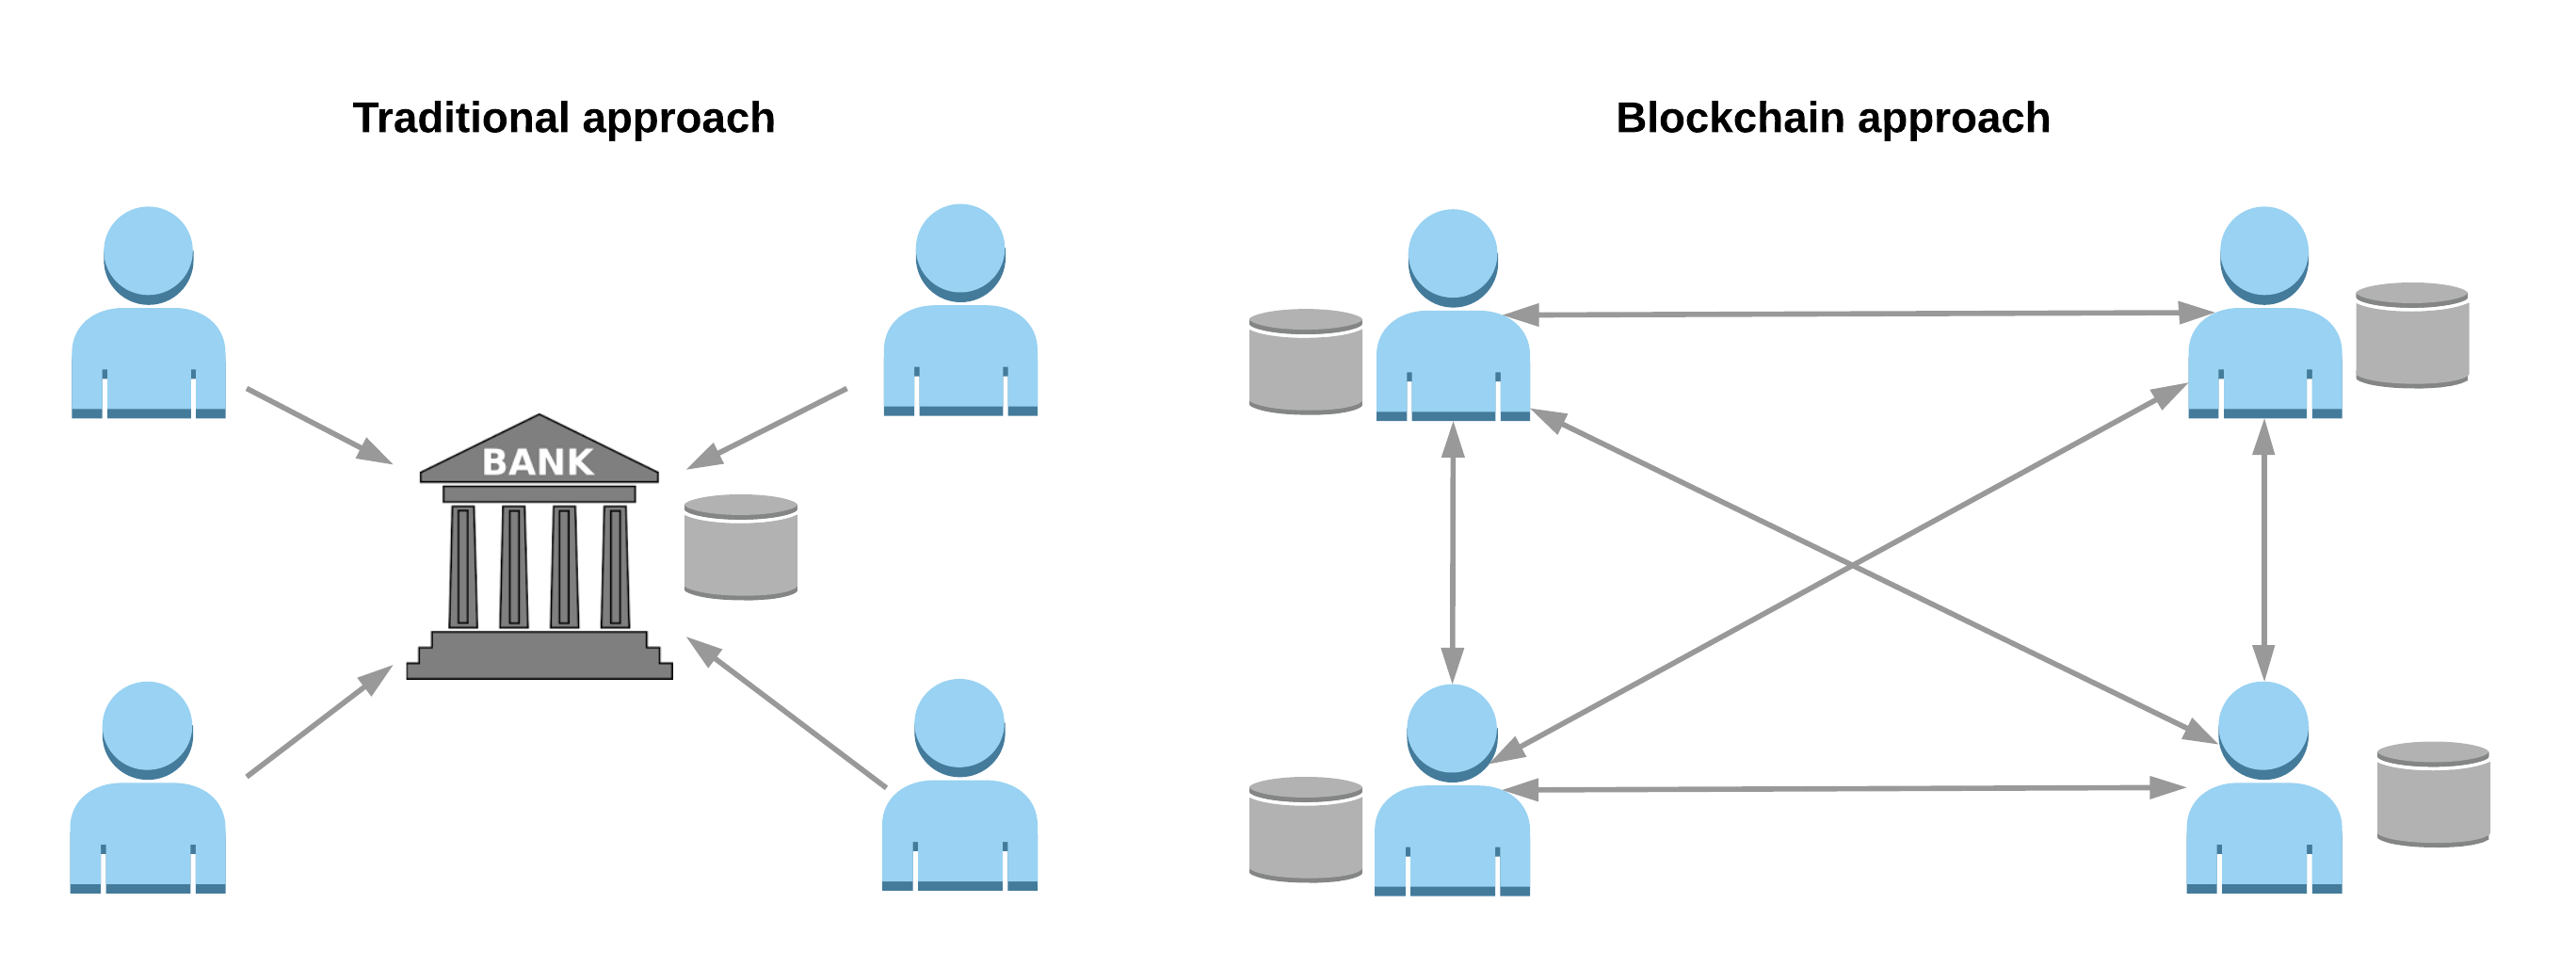
\includegraphics[width=0.8\linewidth]{gfx/cenVsDec}    
  	\caption{Traditional database vs blockchain approach}
  	\label{fig:CentralizedvsDecentralized}
\end{figure}

At the beginning, the terms Bitcoin and blockchain were sometimes interchanged, as these words were used to refer: (i) the technology, (ii) the protocol for making transactions and (iii) the cryptocurrency. Therefore, before continuing, one statement needs to be clear: \textbf{Bitcoin is a cryptocurrency that uses the blockchain technology and cryptocurrencies are just one of the multiple blockchain applications.} 

However, when a new technology appears, the first user's goal is normally to exploit its economic potential. For this reason, money transaction through cryptocurrencies was its first application. In the next subsection, we will understand what cryptocurrencies are, followed by an explanation of the Bitcoin's design architecture.

\subsection{Blockchain 1.0: Cryptocurrencies}

At of the end of January 2018, Coinmarketcap\footnote{https://coinmarketcap.com/}, a cryptocurrency market tracker, lists more than 1,400 cryptocurrencies with an aggregate value approaching USD 700bn. But what are cryptocurrencies? Cryptocurrencies are a variety of digital currencies pretending to work as a medium of exchange, such as Euro or USD does. As the name suggests, apart from being a virtual currency, they use cryptography to secure and verify its transactions. The main difference with traditional currencies is that they do not have any physical equivalent in the real world. Nevertheless, they can be used to pay goods and service, with the advantage of not being constrained with geographical or political borders. For example, GMO Internet\footnote{https://www.gmo.jp/en/}, a Japanese company, will start paying parts of employees salaries in cryptocurrencies (Bitcoin).

In this paper, we will set aside whether cryptocurrencies can become true currencies or not, and also the political, social or economic impact. The only focus will be on the technology behind it, as blockchain can be extended to much more than digital currencies. Thus, we will start from the genesis of the technology, with Bitcoin as its revolutionary innovator.


\subsubsection{Bitcoin}

Bitcoin took the world by surprise in 2008, after Satoshi Nakotomo's white paper publication \cite{nakamoto2008bitcoin} and later its software release. Bitcoin (BTC) is a cryptocurrency used for making secure transactions across a peer-to-peer (P2P) network. In addition, Bitcoin uses its own protocol that operates in an overlay network, the blockchain. An overlay network is a computer network built in the top of another network, in this case above the Internet application layer, which is controlled by its users.

From another point of view, cryptocurrencies ledgers can be interpreted as state transition systems, where there is an initial state that after a transition function (money transfer), results in a new state. In Bitcoin, this initial state is a list of mined but still not spent transactions, each containing also the address supplying BTCs. This transaction output will be the receiving address along with the amount received. For this reason, Bitcoin is considered an unspent transaction output (UTXO) data model. Imagine an scenario where user A wants to send 10 BTC to user B. The first state is A and B current balance, e.g. $\{A = 10, B = 20\}$, and the transition function will take 10 BTC from A and insert it to B's account, generating a new state, now $\{A = 0, B = 30\}$. But what happens if A sends exactly the same payment to two different addresses (B and C) at the same time? This scenario is the so-called \textit{double spending attack} and consequently, a transaction always needs to be verified by miners before being confirmed. 

\paragraph{Mining and Transactions}

Miners are specific blockchain users, responsible for monitoring and verifying all the transactions between users. And how all these miners cooperate efficiently? The answer to this question is one of the most remarkable Satoshi innovation key factors, which consists of the communication between nodes through a simple decentralized consensus protocol. This consensus protocol consists of multiple algorithms (e.g. Proof of Work), used by the miners in the Bitcoin network.

Therefore, Bitcoin needs to combine its chains with a consensus protocol, in order to synchronize the order of all transactions among the users. There, new transactions are stored in the last block of the blockchain, and a new block is mined on average every ten minutes. Over time, this creates an ever-growing chain of blocks, which are constantly updated. Thus the name: blockchain. Additionally, a complete history of the transactions is kept, so everyone can verify the last money movements. For instance, a blockchain can be compared to an endless domino game, where all the pieces are placed in vertical one after the other. Each of these pieces references the previous block, and if one block is removed (e.g. transaction error), all the subsequent ones will be affected. Hence, as miner's task is not simple and requires computational power, if they are the first block solvers, they are also economically rewarded.

Apart from a list of transactions, each Bitcoin block contains a \textbf{block header}, whose hash is stored in the next block in order to maintain a consensus. Figure \ref{fig:Bitcoin Blockchain mining} shows how transactions are bundled into blocks, where each block header contains:

\begin{figure}[t]
  	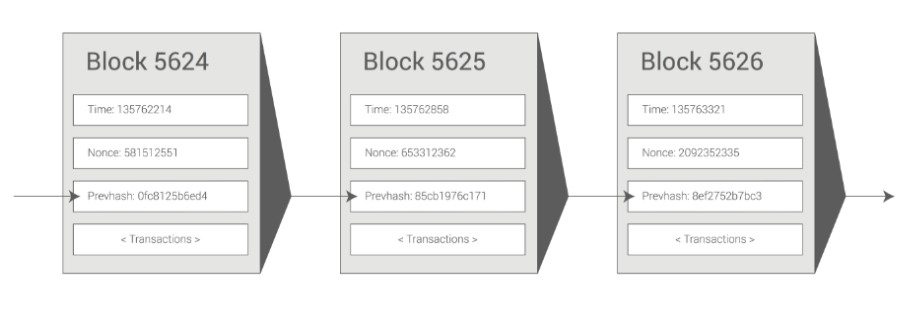
\includegraphics[width=1\linewidth]{gfx/mining}    
  	\caption{Bitcoin blockchain structure. Adapted from \citep{hans2017blockchain}}
  	\label{fig:Bitcoin Blockchain mining}
\end{figure}

\begin{itemize}
	\item A timestamp, to identify when the event occurs.
	\item A nonce, which is an arbitrary number used for the miner to create the block header.
	\item Previous block header hash, to keep track of already added blocks.
	\item A block version number that indicates the validation rules used.
	\item A Nbits field, whose value should be higher than the block's header hash (later explained).
	\item A list of all the transactions that have been created since the previous block. To save storage, this transaction list is typically stored in a Merkle tree, which is a binary tree hash \citep{merkle1987digital}.

\end{itemize}

Furthermore, in Bitcoin, each block and transaction is restricted to a size of 1MB and 250-300bytes respectively, and for a block being valid it needs to satisfy the following requirements:

\begin{itemize}
	\item Previous block referenced exists.
	\item Block's timestamp is greater than previous block one.
	\item Proof-of-work in this block is valid.
	\item If any transaction from the transaction lists returns an error, exit.
	\item If all previous steps confirmed, store state at the end of the block and return true.
\end{itemize}  

In the third step of the block validation process, appears the term \textit{Proof-of-work}. Bitcoin uses the \textit{Hashcash} proof of work algorithm to prove that a block miner spent some computational time creating a block. More precisely, Bitcoin protocol demands that miners find an input, which is a valid $block \, header$ formed by a random value ($c$) and a nonce ($x$), whose cryptographic hash (e.g $SHA256$) is less than a \textit{target} value (non-encoded version of Nbits). This value is obtained from $d$, the blockchain difficulty. Then, the only way to create a valid block is simply trial and error until a valid Proof-of-Work is generated. Proof-of-work is also used in other contexts, such as for limiting email spam or denial-of-service attacks (DoS).

$$ F_d( \, block \, header \,) = F_d( \,c,x \,) = SHA256( \, SHA256( \, c|x \,) \,)\, < \frac{2^{224}}{d}$$

\paragraph{Key management}

In Bitcoin, each user is identified by a single public address. However, how is this Bitcoin address generated? This process involves the following steps:

\begin{enumerate}
	
	\item A random 256-bit private key is created. Since this key will be used to sign the transactions, it must be kept secret.
	\item A 512-bit public key is generated from the private key, using the Elliptic Curve Digital Signature Algorithm (ECDSA\footnote{\url{https://www.maximintegrated.com/en/app-notes/index.mvp/id/5767}}). This key is used for verifying private key signatures.
	\item This public key is hashed to 160 bits using SHA-256/RIPEMD. Apart from size constraints, the reason for hashing the public key is that if there is a vulnerability in elliptic curves, user's money can still be safe, since only the hash is known.
	\item Finally, the public key is encoded in ASCII using Base58Check. This output is the resulting Bitcoin address.
	
\end{enumerate}

\begin{figure}[bth]
  \centering
  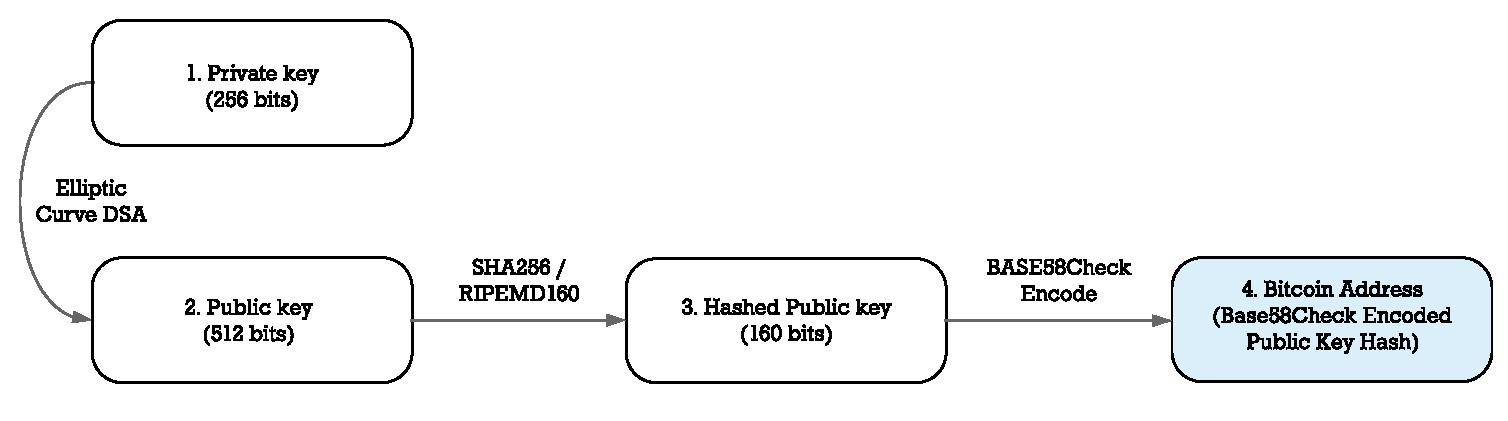
\includegraphics[width=0.9\linewidth]{gfx/bitkeys}    
  \caption{Bitcoin keys and addresses generation \citep{BitcoinKey2018}}
  \label{fig:EthereumAccounts}
\end{figure}

After that, users are able to send transactions using Bitcoin. For example, imagine the last example where user A wants to send 10 BTC to user B. Firstly, the user creates a transaction willing to transfer 10 BTC to user address B. Secondly, he signs the transaction with his private key, attaching also his public key, and sends it to the blockchain. There, miners will verify the signature using A's public key and also that its hash matches user A address. If both, the signature and the hash, are correct, the transaction is accepted and added to the next block. Transaction examples can be found in Block Explorer\footnote{\url{https://blockexplorer.com/}}.

\subsection{Blockchain 2.0: Smart contracts} \label{smartContracts}

The Blockchain 1.0 had numerous limitations since essentially it only approaches the decentralization of money and payments. However, the architecture implemented by Bitcoin is extensible beyond financial uses cases.

\subsubsection{Ethereum}

In 2013 Vitalik Buterin, a Russian-Canadian programmer released the Ethereum white paper \cite{buterin2014next}, where he describes an alternative platform running in a blockchain that allows building any kind of decentralized applications. In 2014, Gavin Wood published the Ethereum
yellow paper introducing the Ethereum Virtual Machine (EVM), i.e. a blockchain with a built-in programming language. Ethereum first started as a crowdfunding project, which collects small amounts of money from a large number of users. Currently, Ethereum is the second most valuable cryptocurrency.

Furthermore, it extends the power of decentralized transactions with a Turing-complete contract system. A Turing-complete system can be proven mathematically to be capable of performing any computation, which allows developers to create its own programs. The code of these functions are written into the so-called \textbf{smart contracts} and executed by the Ethereum nodes, each using its Ethereum Virtual Machine (EVM).

In the end, smart contracts are basically Ethereum scripts that whenever they are called, the function programmed inside of it is executed. A simple example of a contract is the logic inside a vending machine. For instance, a buyer wants a Coke bottle that costs 2 \euro. Once this buyer inserts 2 \euro and presses the button, a small program (contract) runs inside the vending machine and supplies the user with the Coke. This function, in the smart contract context can be seen as:

\begin{lstlisting}
contract Products {

	function getItem(bytes32 buttonPressed, uint amount) returns(bytes32 item) {
		if (buttonPressed == 'coke' && amount == 2) return coke;
 		return null;
	}
}
\end{lstlisting}

Therefore, smart contracts allow anyone to write their own functions, in just a few lines of code. Despite the fact that Bitcoin and Ethereum have similar features, such as decentralization or being transaction-based, Ethereum makes use of smart contracts, which potentially opens up real-world use cases. Bitcoin and Ethereum can be comparable to a calculator (one application) and a smartphone (multiple applications) respectively. In addition to the already mentioned differences, there are other inequalities that need to be highlighted:

\begin{itemize}
	
	\item Ethereum's block time is shorter, specifically it is around 14s. Remember that Bitcoin's mining time was around 10 minutes. Hence, as a consequence, Ethereum needs to handle large amounts of transactions per seconds, which means that the network can easily get separated in different subchains. To solve these scalability issues, \textit{Casper}, a protocol from the new \textit{Proof-of-Stake} (PoS) mechanism has been recently proposed \cite{proofOfStake}.
	\item Thus, Ethereum pretends to move from the \textit{Proof-of-Work} to the \textit{Proof-of-Stake} consensus algorithm. In contrast to PoW, where the miners that first solve a mathematical problem are rewarded, in PoS, validators propose and vote the next block. The voting power is directly proportional to the validator's stake (deposit). To become validators, users need to lock up their ether into a deposit. Therefore, in PoS there are validators rather than miners.
	\item Bitcoin's blocks and transaction sizes are indicated in bytes, however, in Ethereum, this depends on the contract complexity. This complexity is expressed in terms of \textit{gas}, which is the amount of \textit{ether}\footnote{\textit{ether} or ETH is the digital currency used by Ethereum}, used for executing contracts in the Ethereum blockchain. 

	\item Ethereum transactions compared to the mentioned Bitcoin fields consists of (i) the transaction value in Ether, (ii) recipient address, (iii) data arguments and (iv) execution cost.
	\item Ethereum is account-based and not transaction-based.
\end{itemize}
Also, a miner does not receive a block reward, but instead he earns all gas used for executing the smart contract.
In the last point, we observe that Ethereum introduces a new concept called accounts. These accounts are unique 20-byte addresses in the blockchain, each of them having a balance controlled by ethers (ETHs). In Ethereum, there are two types of accounts (Figure \ref{fig:EthereumAccounts}):

\begin{itemize}
	
	\item \textbf{Externally Owned Accounts (EOAs):} These accounts identify users while being controlled by their own public and private keys. Only EOA can send transactions to other accounts. A transaction in Ethereum can either send Ethers or call/trigger a contract account  
	\item \textbf{Contract accounts:} These are the accounts, where the code (smart contract) is stored. Thus, once triggered (function call from another contract), its defined code is executed.
\end{itemize}

\begin{figure}[bth]
  \centering
  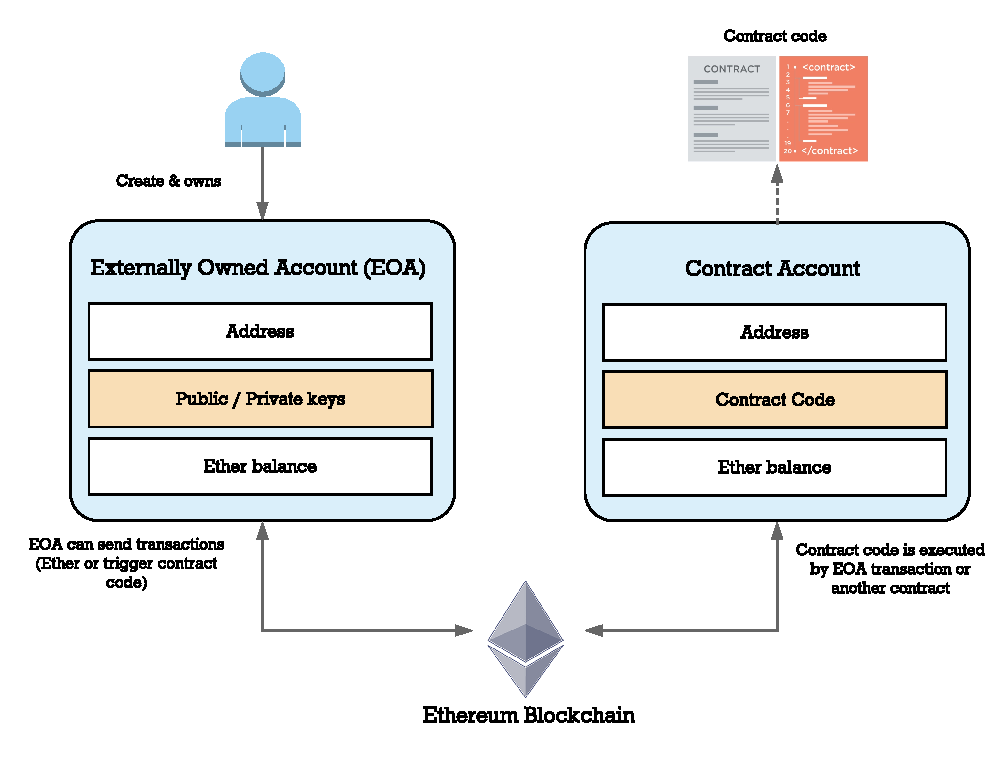
\includegraphics[width=0.6\linewidth]{gfx/ethereumAccounts}    
  \caption{Ethereum accounts: Externally owned accounts and contract 			accounts}
  \label{fig:EthereumAccounts}
\end{figure}

However, what happens if this contract code results in an infinite loop?Ethereum solves this using gas. For example, suppose an EOA calling a contract account for money transfer. Apart from the ether transferred, it will also spend an additional amount of ether (gas). Thus, the ether used for a transaction, or transaction fee $F$ is:

$$F = P \times L + V - R$$

Firstly, the gas limit $L$ is the maximum amount of gas to spend on a transaction, which is by default 21000. Secondly, on Ethereum the gas price $P$ is measured in units of Gwei, which is equivalent to $1e^{-9}$ ETH. Thirdly, the value $V$ is the amount of ether transferred to the other EOA. Fortunately, all unused gas $R$ during a transaction is refunded to the sender. Nevertheless, if a transaction returns an error, e.g: gas provided not enough to execute a contract, this provided ether will never be refunded. 

In conclusion, a smart contact is just an account containing code, which lives on the blockchain and allows developers to create their own decentralized applications. 

\subsubsection{Decentralized applications}

In the Ethereum white paper \cite{buterin2014next} decentralized applications DAPPs are split into three types. The first group includes financial applications, where users only want to manage money transactions, e.g. a customer paying the provider through a blockchain application. The second group is formed by semi-financial applications, in which money is involved but it is mixed with other requirements. For instance, an application where users receive incentives when solutions to computational problems are provided. And finally, in the third category, there are non-financial applications. For instance, an online voting platform providing a better transparency into elections, without compromising voter confidentiality.

Despite the blockchain is a secure technology, the created applications are constantly compromised to multiple attacks. This is because the majority of smart contracts are insecure, due to its code being prone to bugs.
For example, in June 2016, the DAO\footnote{https://ethereum.org/dao}, a distributed autonomous organization instantiated on the Ethereum blockchain, was hacked. The attack, which was a smart contract bug, had resulted in over 50 million dollars of cryptocurrency theft. Thus, smart contracts need to be protected against malicious attacks before being uploaded on the blockchain.

In the following section, an example application or process currently performed by IT companies will be introduced.


\section{Network Virtualization} \label{networkvirtualization}

In the last few years, network virtualization has started to grow in popularity since it enables simulating hardware networks. These virtual networks, in contrast to physical networks, provide flexibility, manageability and a low cost. 

Network virtualization handles two main concepts: node virtualization and link virtualization. The former implies sharing the node's physical resources located in the substrate network (e.g: CPU, storage, memory) to multiple virtual nodes in the virtual networks, such as physical node A in Figure \ref{fig:networkvir}.a. The latter enables the transport of multiple virtual links in a single and shared physical link (Figure \ref{fig:networkvir}.b).

\begin{figure}[bth]
  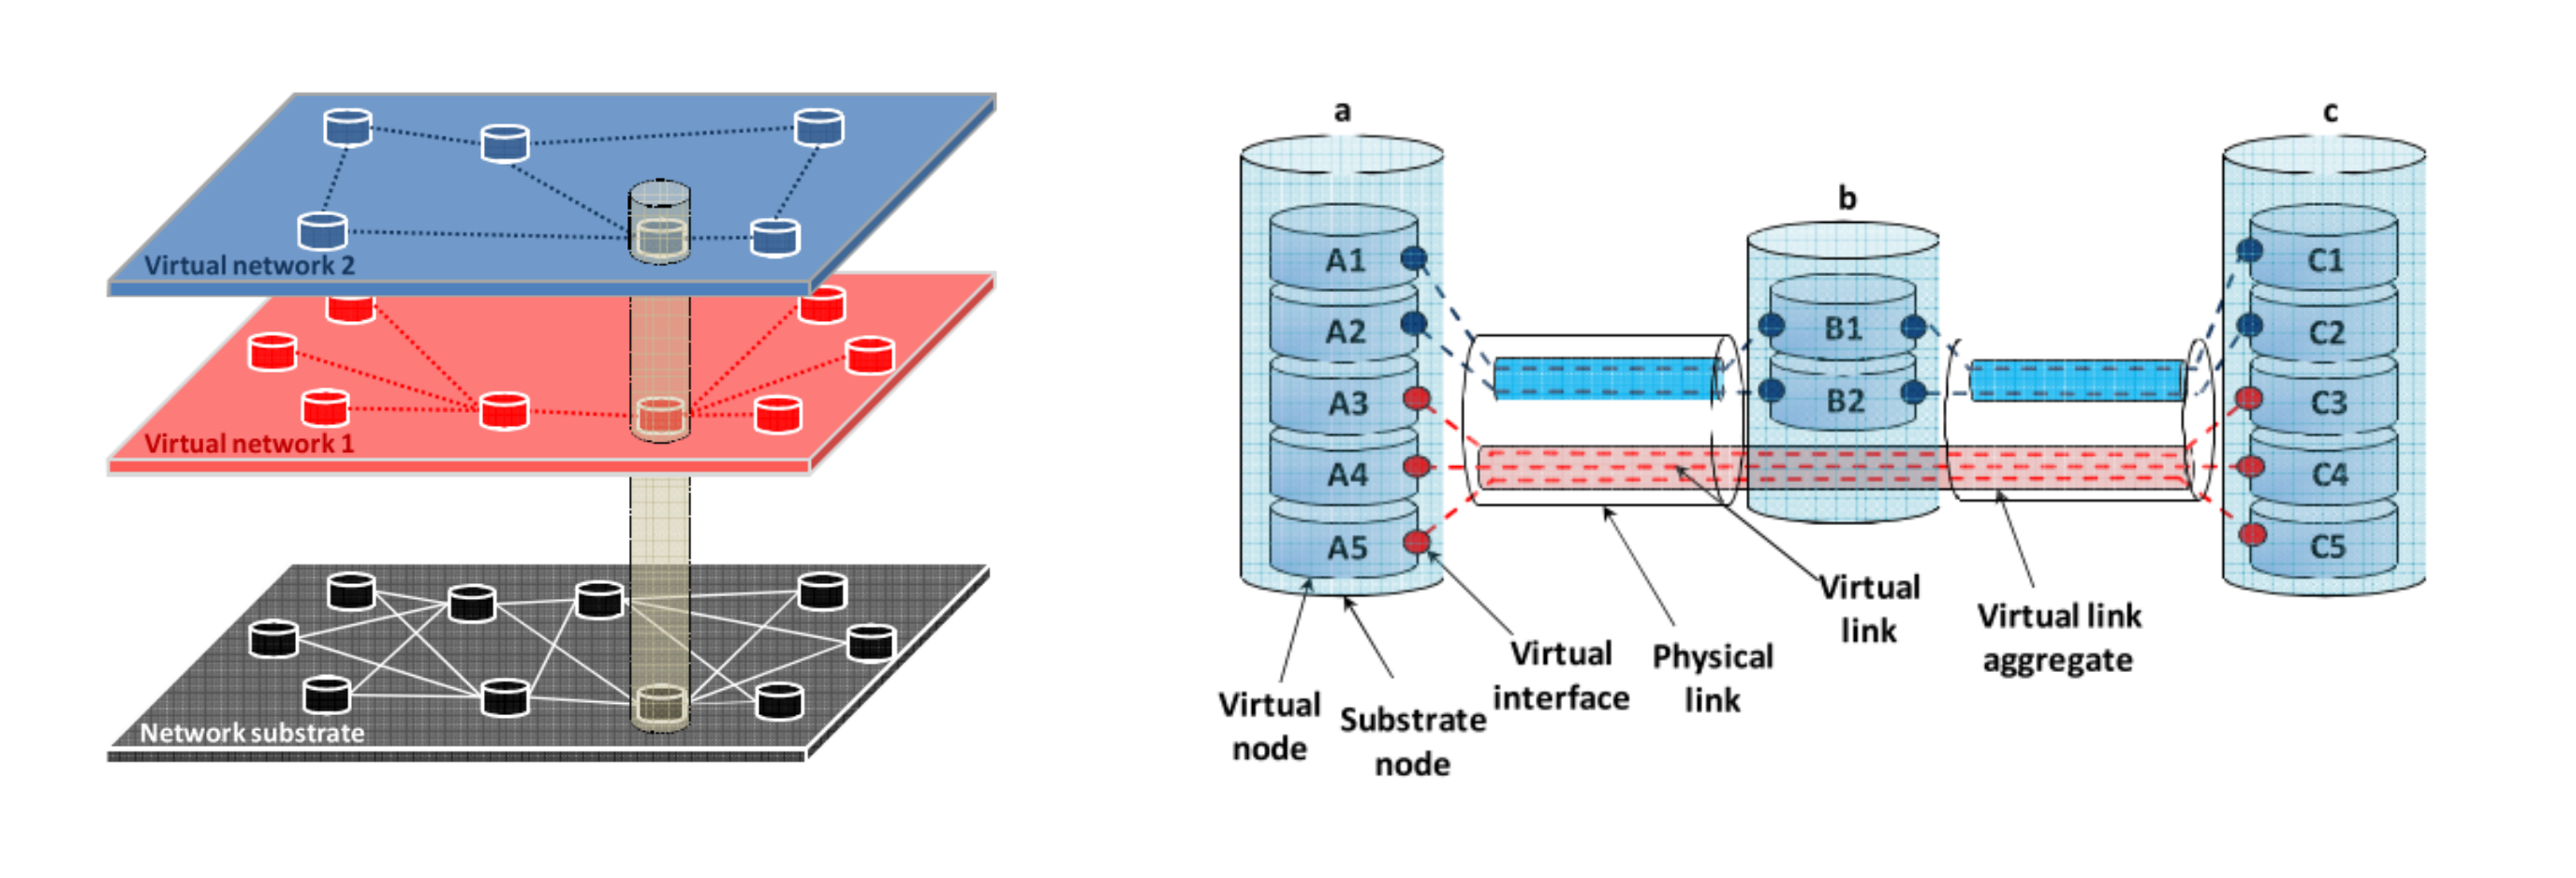
\includegraphics[width=1\linewidth]{gfx/networkvir}    
  \caption{Network virtualization model and its basic elements \citep{carapinha2009network}}
  \label{fig:networkvir}
\end{figure}

In a real scenario, there are two main actors (and one optional) participating in the network virtualization process.

\begin{itemize}
	
	\item \textbf{Infrastructure providers (InPs):} Infrastructure providers (e.g: Deutsche Telekom or Telefonica) deploy and manage the physical nodes, sharing efficiently its resources to the virtual network. For InPs, this results in a significant decrease in operational and technology investment costs \citep{dietrich2015multi}.
	\item \textbf{Service Providers (SPs):} Service providers lease virtual resources from infrastructure providers to create its customized virtual network. This is done without the need to purchase physical network equipment.
		\item \textbf{Virtual network providers (VNPs):} Are brokers, which can optionally serve as intermediaries between the infrastructure providers and service providers.
\end{itemize}

The network slicing process with the presence of a broker typically starts with the VNP obtaining the necessary network information from the SP. To optimize the software costs, the SP's virtual network request will be divided into groups of nodes (subgraphs). Afterwards, the modified network is transmitted to the multiple InPs, who are in charge of embedding the virtual nodes from the request in their physical resources. 

The presented process is coordinated by an actor, the VNP, who stores all the network information to successfully allocate the incoming resources. However, there are other approaches, where the InPs do not want to rely on a central entity, since its confidential information is being disclosed and hence, known by the VNP. Conversely, the SPs and InPs make use of consensus mechanisms to perform the virtual resources trading. Thus, the network virtualization task is accomplished in a more decentralized manner, since no middle-party exists. In the following, we will briefly investigate an open negotiation technique: the auctions.

\subsection{Auction Mechanisms} \label{auctionMechanisms}

Service negotiation has already been examined in many researchs, such as \citep{hausheer2005peermart}, \cite{ogston2002peer}, which have worked with diverse auctions platforms. An auction is a public negotiation method involving buyers and sellers that enables resource trading between peer-to-peer users. While the buyer's goal is to find the desired service at the lowest price, the providers or seller's goal is to sell the service at the highest "possible" price. Thus, an auction must provide fairness in terms of technical and economic efficiency, for both the buyer and the seller.

Firstly, auctions can be divided into (i) \textit{one-sided auctions} where only the buyers submit their bids (e.g: a painting auctioned in an art exhibition), or (ii) \textit{two-sided auctions} in which buyers and sellers submit their bids. Normally, when any of the two sides (buyer or seller) cannot perform a good estimation of the service, a one-side auction is preferred. This is the case in network virtualization, where the SPs are not aware of the InPs physical nodes availability or complexity. Secondly, the auctions can be (i) \textit{open-cry} auctions, where the bids are broadcasted to all users, or (ii) \textit{sealed-bid} auctions in which bidders first commit bid values in secret that are later revealed (e.g: physical envelopes). In our scenario, the InPs should bid in a confidential manner, because they do not want to disclose internal network cost models. In addition, concerning auction types, our focus will be on the most common \cite{coppinger1980incentives}: 

\begin{itemize}
	\item \textbf{English auctions}, also called \textit{open-cry ascending-price} auction, is the classic bidding mechanism where the seller first sets a minimum starting value (reserve price), which buyers should overcome. Then, these buyers start to offer higher prices until nobody wants to offer a greater one. However, due to the competition, this auction model can result in a long process (e.g. low reserve price compared to real value) where users pay huge amounts.
	\item \textbf{Dutch auctions} are similar to the English auctions, but on the contrary, they are \textit{open-cry descending-price} auctions. In this model, seller fixes a maximum value which is reduced slightly over time. Once a buyer accepts a price, the auction will finish. Nevertheless, to prevent ending with low prices for the sellers, they also establish the mentioned reserve price, which will be the minimum accepted amount. Dutch auctions are faster than the English ones, but buyers will also end up paying more to ensure that they win.
	\item \textbf{Vickrey auctions} \cite{vickrey1961counterspeculation} has the particularity of corresponding to a \textit{sealed-bid second-price} auction. Since it is sealed, during the bidding time buyers do not know other bids and eventually, how the auction is evolving. In addition, the Vickrey auction corresponds to a second-price tender. This means that like standard auctions, the bidders will offer a price for the service, and the highest bid will win. Nevertheless, this service will be rendered at the second highest value. For example, imagine a bidding for product A, where the winner has bidden $\{A = 15\}$ and the second highest bid is $\{A = 10\}$. Then, this winner ends-up paying only $\{A = 10\}$. In addition, it is shown that a Vickrey auction is strategy-proof \cite{vickrey1961counterspeculation}, meaning that each bidder quotes the true cost of the service, and if they do so, the resulting total values are maximised. From the bidder's point of view this means that he can safely bid the real value, knowing that if he wins, he will pay less than his bid. Thus, a Vickrey auction compared to English and Dutch auctions, is considered a fair-price system since it provides a reasonable price to the buyer by motivating bidders to bid truthfully.
	\item \textbf{Reverse auctions} as the name states, buyers and sellers roles are switched. In contrast to ordinary auctions, where buyers compete to obtain an asset, in reverse auctions, sellers compete to gain a business. In other words, the seller bids for his own provided services, which in the end, will be given to the supplier offering the lowest price. For example, in the network virtualization process, InPs will bid for the lease of their physical nodes, and afterwards, the SP will rent the most economical ones.
\end{itemize}

Ultimately, after judging the preceding analysis regarding auction types, a \textbf{\textit{one-sided reverse Vickrey}} auction seems to be the most suitable for network virtualization since it provides confidentiality and the biggest aggregate profit among sellers and buyers. This will be later investigated in section \ref{ch:design}.

\section{Summary}

The blockchain is a transparent, secure and robust system where users are in charge of their own accounts and transactions. Beyond money transfer, which started with Bitcoin, the blockchain technology can be used as a software connector in multiple scenarios. Due to smart contracts, arbitrary applications could be implemented in the context of Ethereum blockchains, enabling developers using the blockchain concept in their own environment. In the next chapters, we will investigate a multi-provider virtual network embedding scenario where infrastructure providers are not willing to disclose internal network cost models.

%*****************************************
\chapter{Related Work}
\label{ch:relatedwork}
%*****************************************

In the following, we explore some of the noted challenges that organizations encounter during their supply chain management (SCM) process, and how they currently approach these issues. Then, we will introduce a recent application in manufacturing, to demonstrate how blockchain could improve SCM efficiency. Henceforth, we focus on a particular supply chain management example: virtual network embedding across multiple InPs. A comprehensive overview of related work on already implemented centralized and decentralized frameworks will be presented. Finally, we will first enumerate the main blockchain benefits observed from the SCM manufacturing application point of view, and secondly, we will analyze the pros and cons of the existing VNE related work, in order to observe the problems and limitations that need to be addressed in our thesis.

\section{Blockchain in Supply Chain Management}

In the last years, managing the information during the lifecycle of a product represented a major challenge for many companies \citep{karkkainen2003product}, \citep{tuttle2002you}. This product information is constantly changing and in addition, it has to be accessible by different entities. As a consequence, this problem results in high costs for companies. 

Typically, companies approach the problem in the following way: (i) storing and maintaining its data into their company-specific infrastructures, which is then communicated to the other supply chain partners, or (ii) sharing this data in a centralized database. In the former, each enterprise creates its own copy of the product data, using their own protocols and procedures.  As a consequence, a lot of information asymmetries are found, which ends up destroying the benefits of knowledge or data sharing. In \citep{lee1992managing} and \citep{fiala2005information} inadequate definition of customer services, poor coordination or organizational barriers are named to be some of the pitfalls that these users suffer from. On the other hand, the latter is a great solution as long as the companies trust the party who is maintaining the database. However, what if they are not willing to place this intermediary on their operations? Here, we foresee that blockchain could improve the process supplying data distribution and storage among these companies.

Apart from the supply chain, \citep{heikkila2002supply} states another relationship between suppliers and customers, the Demand Chain Management (DCM), where we predict that blockchain could also play a significant role. In a DCM, the aim is to provide a customer service at the least cost. Hence, the suppliers need a real-time visibility of customer situations and needs. The main difference is that in SCM, the stakeholders wait to receive the order for proceeding with a product (push), whereas in DCM the suppliers observe and immediately operate in user's petition (pull) \citep{wust2017you}. Currently, companies such as Everledger or Skuchain\footnote{\url{http://www.skuchain.com/}}, offer blockchain services to manage and improve the supply chain performance.
 
In the following section, a blockchain application for a manufacturing supply chain system will be presented.

\subsection{Blockchain Ready Manufacturing Supply Chain} \label{manufacturing}

In this part, a blockchain example \citep{abeyratne2016blockchain}, which stores and distributes specific product information during its lifecycle, will be discussed. This task also named product lifecycle management (PLM), involves different stages \citep{stark2015product}, in which multiple parties modify the product's data, see Figure \ref{fig:supplyChain}.a. In this scenario, each actor interacts with a user interface, which is connected to the product's data from the blockchain. Each product is created in form of rules (smart contract) so that only specific users can access or modify the information. To access or alter this data, parties must authenticate themselves signing the requests with their private keys. 

During the lifecycle management, a product is owned by an entity, for instance the distributors. Moreover, when a product goes to another actor (e.g. from distributors to a consumer), both parties will sign a contract that updates product's ownership. Thus, the system ensures that in each phase, only the granted user modifies the contract.

At the end of \citep{abeyratne2016blockchain}, an example to better explain the mentioned approach is also presented. The application consists of the product lifecycle of a cardboard box, starting from the trees cut down until the box is recycled. In Figure \ref{fig:supplyChain}.b an overview of the implemented design is presented. In this business process, different actors are entailed. For instance, the box manufacturer first receives the physical object and then signs a contract to gain the product's access. Afterwards, he is allowed to alter it through the user interface (e.g. modify the box quality). Once finished, he will transfer the package (signed) to the next actor, in particular, the product filler, who will follow the same steps.

\begin{figure}
	\centering
	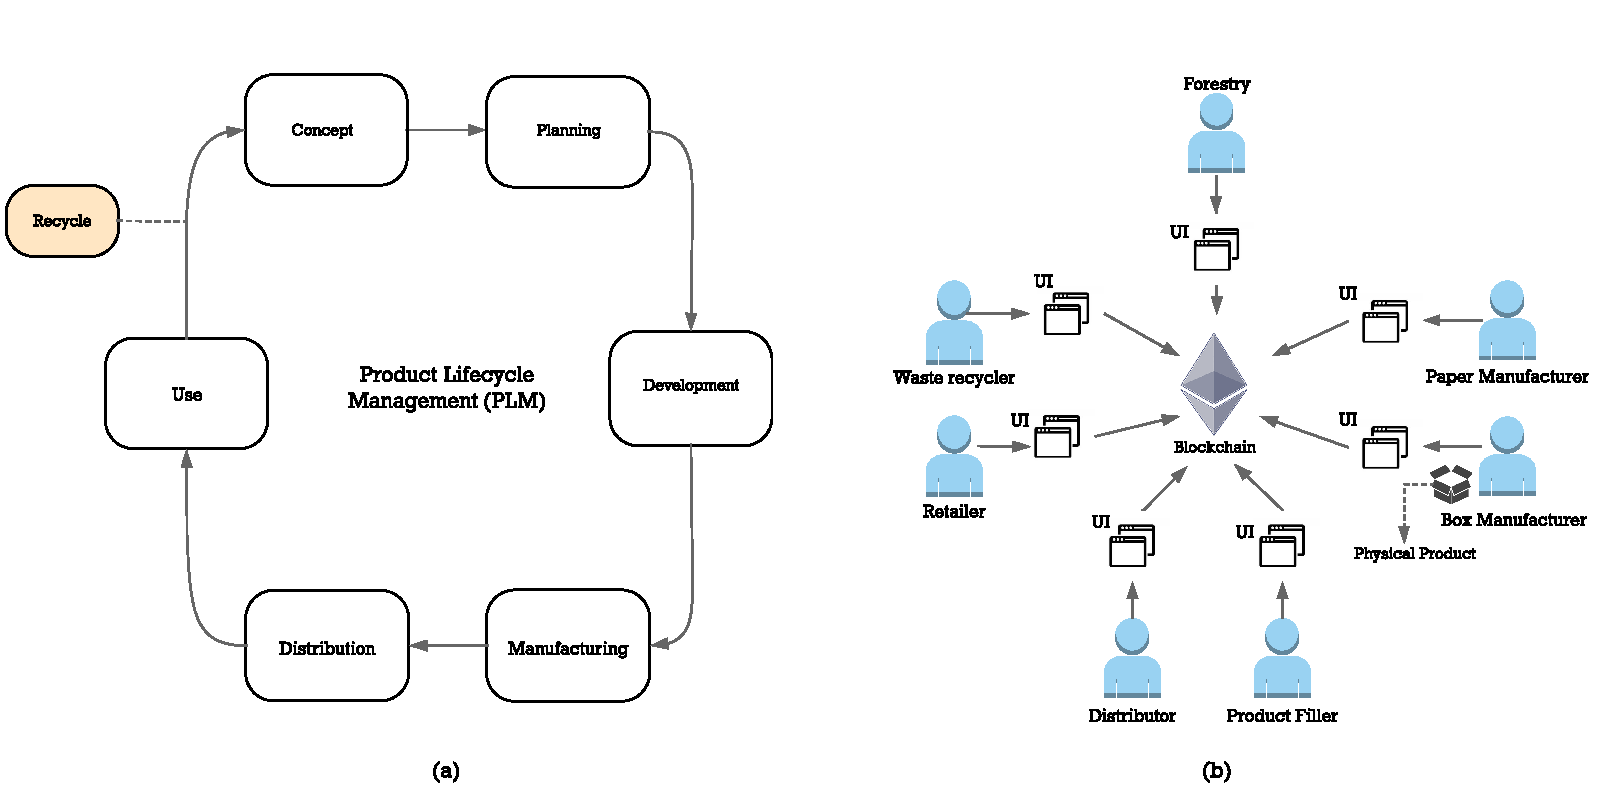
\includegraphics[width=1\linewidth]{gfx/supplyChain}    
  \caption{ PLM stages and cardbox blockchain application example \citep{stark2015product}}
  \label{fig:supplyChain}
\end{figure}

\section{Network virtualization}

In the last years, many investigations in network virtualization have been conducted by different authors \citep{houidi2011virtual}, \citep{zhu2008cabernet}, \citep{chowdhury2009virtual}. Among these, it is important to highlight topics such as the trade-offs between single \citep{chowdhury2009virtual}, \citep{houidi2008distributed} and multi-provider VNE \citep{dietrich2017multi}, or the different techniques and algorithms used for achieving VN efficiency. Typically, they decompose the VNE into two tasks: VN partitioning and VN segment mapping \citep{fischer2013virtual}. 

Each of these studies proposes new interesting features compared to the prior research. Nevertheless, in this paper, we will not contrast the different architectures (e.g. between a single or multiple InPs) or discuss the various VN partitioning and mapping algorithms. The main goal of this work will be to explore an existing network virtualization scenario, in particular, multi-provider VNE applications suffering from the limited information disclosure problem or LID \citep{dietrich2017multi}, \citep{zaheer2010multi}, \citep{esposito2013general}, \citep{chowdhury2010polyvine}.

\subsection{Multi-Provider Virtual Network Embedding with Limited Information Disclosure}

To deploy wide-area networks, service providers are willing to embed virtual resources across heteregeneous domains belonging to different infrastructure providers. As a result, the system avoids being restricted to just a single provider topology, providing at the same time better efficiency. This process, also named inter-domain VNE\footnote{inter-domain is between multiple InPs and intra-domain is inside a single InP.}, is descomposed in three main tasks \citep{chowdhury2010polyvine}:

\begin{itemize}
	\item \textbf{VN request partitioning}: Divide the virtual network into groups of virtual nodes (subgraphs), such that virtual node and link requirements are satisfied, minimizing at the same time the software cost of the virtual network setup.
		\item \textbf{Inter-connection between subgraphs}: Establish paths between the previously created subgraphs.
	\item \textbf{VN segment mapping}: Embed the virtual resources (subgraphs) to the InPs physical nodes.
\end{itemize}

Furthemore, in such scenarios exists two types of communication \citep{zaheer2010multi}:

\begin{itemize}	
	\item \textbf{Horizontal communication} is the one established between infrastructure providers to guarantee the most efficient end-services. These relations can be: \textit{public relations} established using a market mechanism (e.g: an auction), or \textit{private relations} that are previously arranged, because the InPs already know each other. In both cases, the relation arises from the need to negotiate and cooperate to serve the SPs.
	\item \textbf{Vertical communication}, which emerges from the negotiation between SPs and InPs, where the former is willing to lease some virtual resources from the latter. This communication is typically facilitated by a third party (VNP).
\end{itemize}

One of the main challenges of inter-domain VNE, is that InPs are not willing to broadcast their resources information (e.g: nodes availability, cost) or their network topology to the outside world \citep{dietrich2015multi}. Thus, the virtual resources need to be allocated in a constrained and limited scenario (LID). And if that was not enough, this InP's data is crucial to perform the partitioning of resources, in order to optimize the network software costs.

\subsubsection{Centralized Slice Embedding}

In \citep{dietrich2015multi}, a centralized VNE framework is implemented (Figure \ref{fig:multiprov}.a). There, the mentioned LID partitioning problem is approached through a VPN, who accesses public information that is not considered confidential by the InPs:

\begin{itemize}
	\item \textbf{Virtual resources availability}: In this case, virtual resources examples are obtained from Amazon EC2 \cite{amazonEC2}, which announces the attributes (CPU, memory, cost) of different instances types.
	\item \textbf{Substrate network topology}: Most of network's topology information is treated confidentially for the InPs. Nevertheless, there are certain aspects of the network which are not considered private, such as InPs peerings (including location) and its related link cost (Figure \ref{fig:multiprov}.b).
\end{itemize}

\begin{figure}
	\centering
	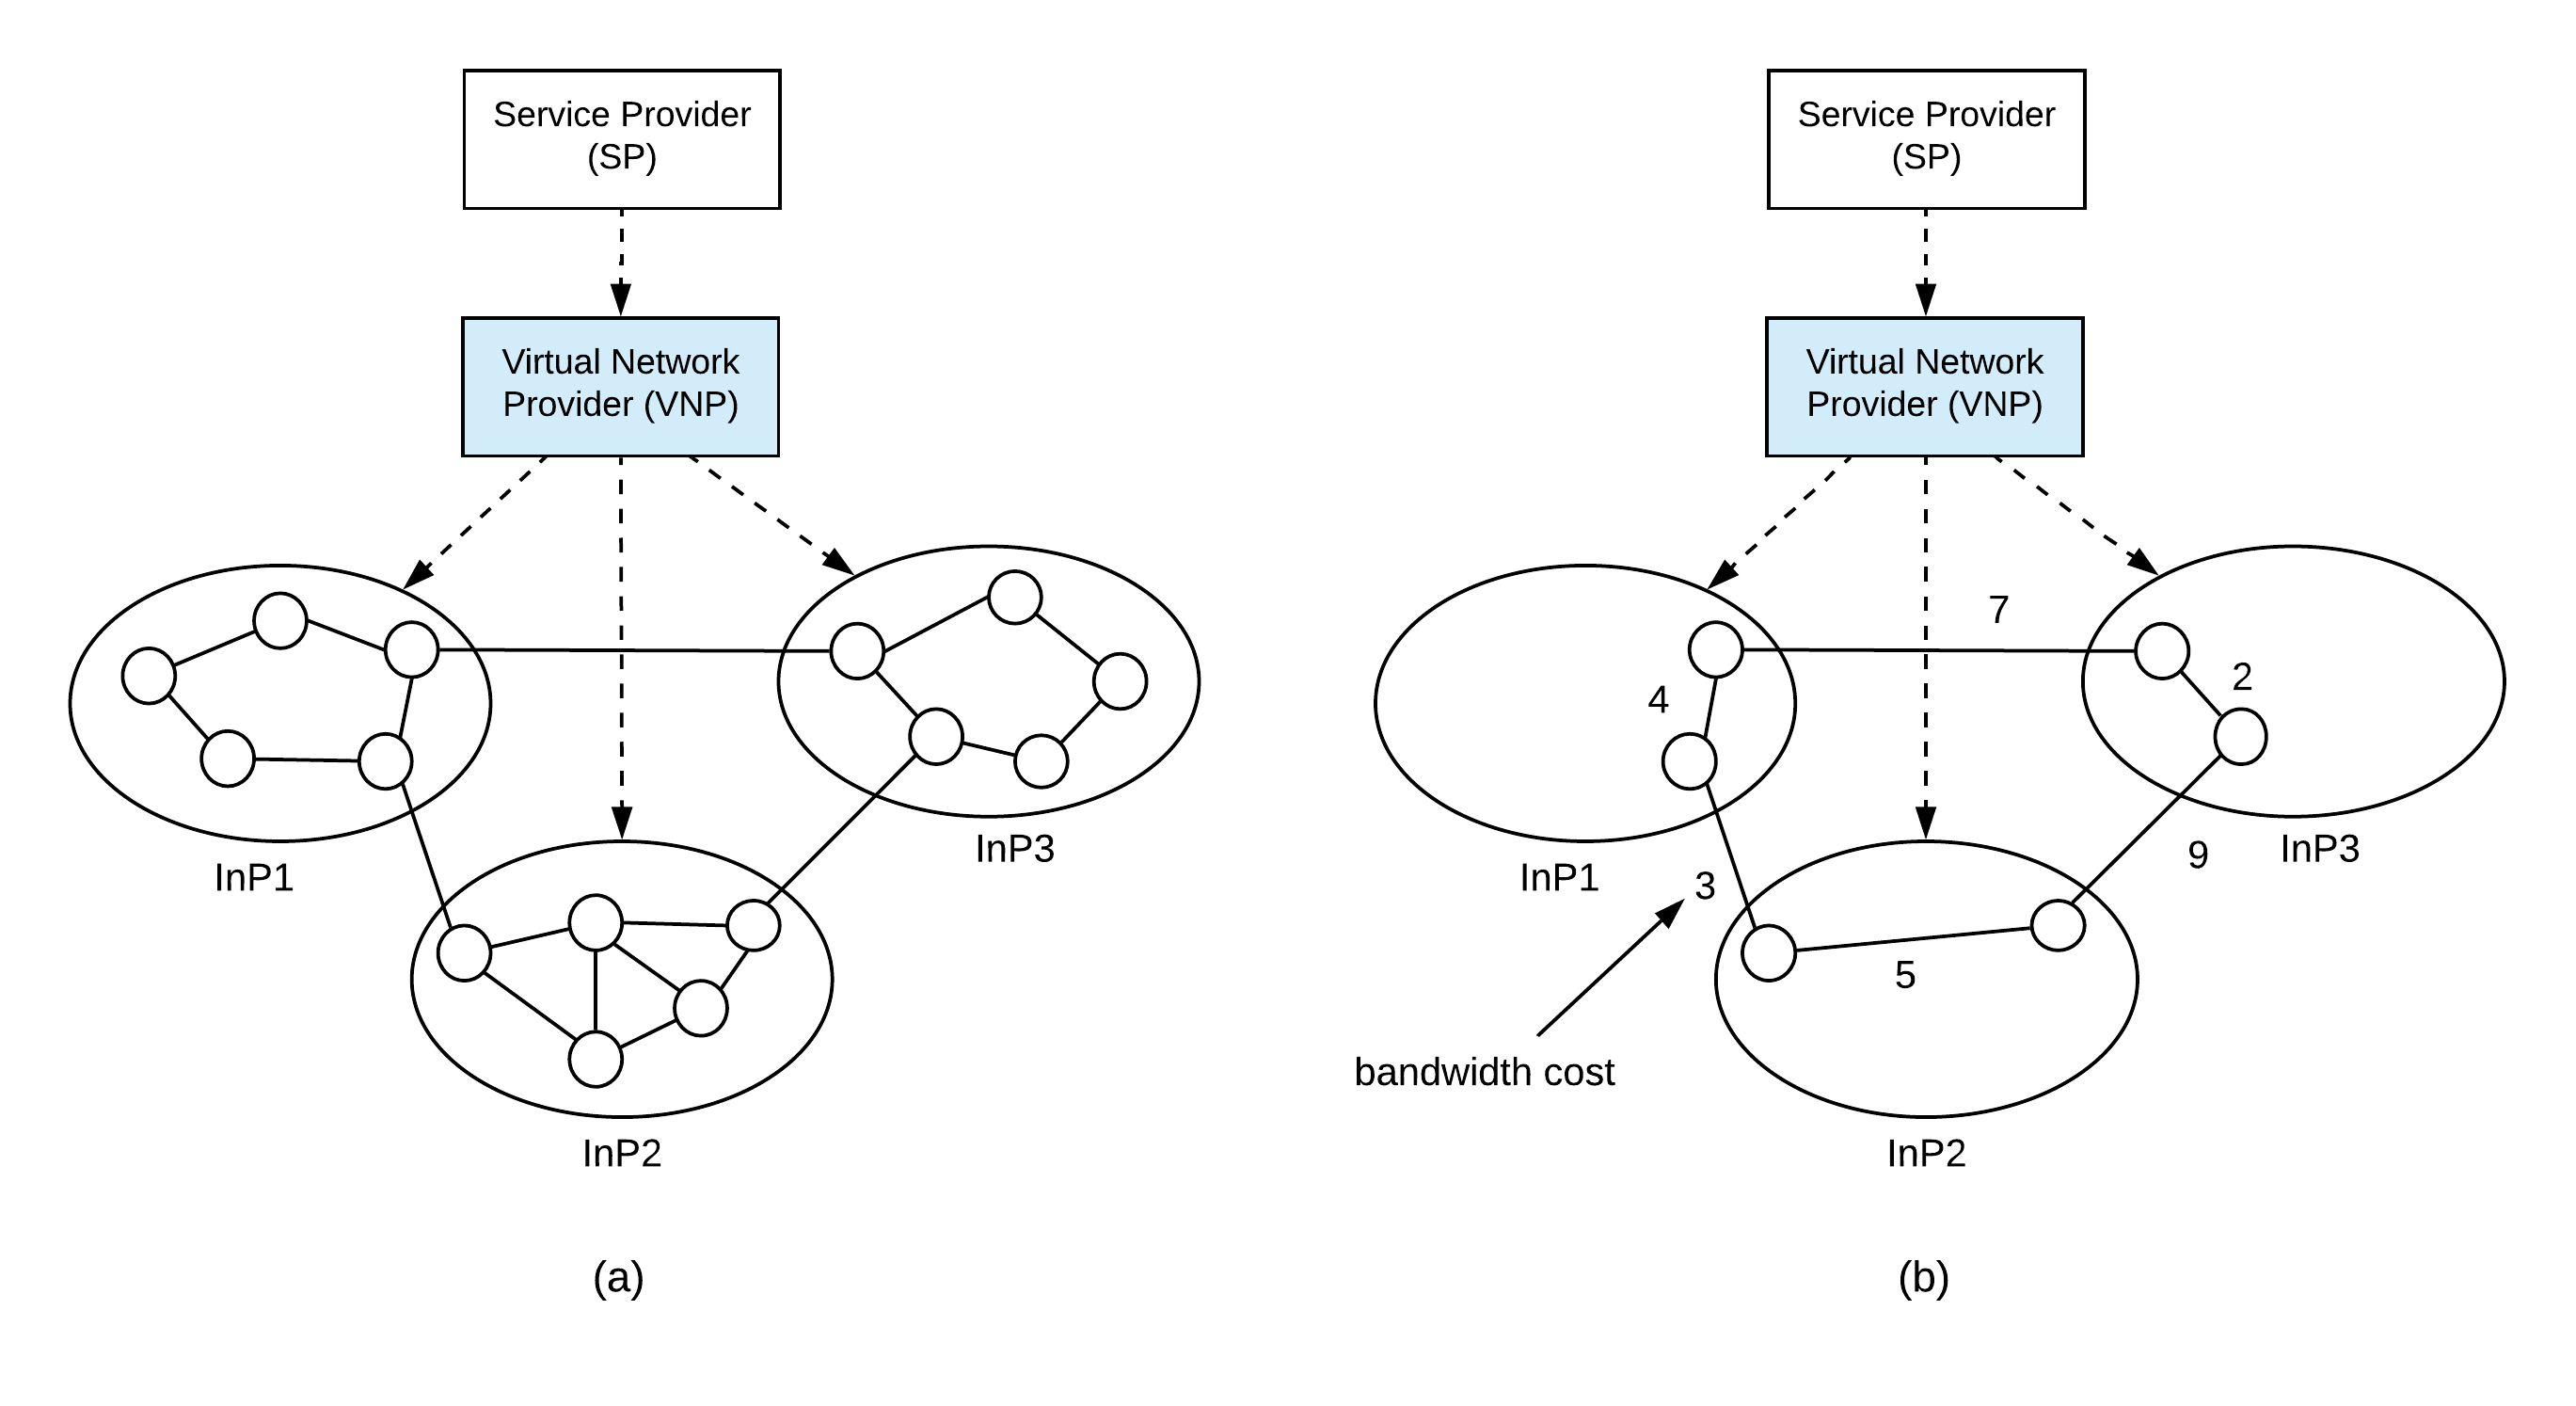
\includegraphics[width=0.9\linewidth]{gfx/multiprov}    
  \caption{(a) Virtual network request across multiple InPs using a VN Provider. (b) VNP's view on the substrate network topologies. \citep{dietrich2015multi}}
  \label{fig:multiprov}
\end{figure}

Furthermore, in the \citep{dietrich2015multi} implemented framework, the slice embedding is achieved by subsequently perfoming the following tasks: Firstly, the above-mentioned resource information is sent from the InPs to the VNP, who registers and stores it. Secondly, the VNP matches the service provider request with this collected data. Thirdly, the corresponding partitioning and mapping algorithms are applied (not discussed in this paper). 

In addition, the results prove that this centralized VNE approach provides embedding costs not much higher than in an ideal case scenario (InPs announcing all required information) and a high ratio between the number of slices requested and later allocated. Despite the positive findings, this scenario suffers mainly from scalability, since everything relies on a single centralized authority: the virtual network provider. In addition, it assumes that InPs (if they do so) will be constantly advertising their updated data to the VNP, which can lead to undesired costs.

Therefore, other approaches where the actors benefit from a more scalable and distributed slice embedding need to be further investigated.

\subsubsection{Distributed Slice Embedding}

Many existing solutions \citep{houidi2011virtual}, \citep{dietrich2015multi}, \citep{dietrich2017multi} rely on a centralized party (VNP) that stores the InPs disclosed information and then performs the partition of the virtual network request. However, what if the SPs and InPs are not willing to trust a centralized broker? In that case, this central actor could be removed enabling a direct communication between the SPs and InPs, which provides a better system scalability. Distributed network slice embedding has already been investigated in:

\begin{itemize}
	\item In \citep{esposito2013general}, a \textbf{consensus-based auction for distributed slice embedding (CAD)} is proposed. In particular, the physical nodes, which are owned by a single or different InPs, bid on virtual nodes. This value is subsequently stored in a vector $b_i$, where $i$ is the physical node. Afterwards, once the bidding phase concludes, each physical node exchange the bids with its neighbors to reach an agreement for the auctioned virtual nodes. The mentioned bidding can be for a single slice (2 virtual nodes and 1 link) or on the entire slice (multiple virtual nodes and links). In the former, there is a limit on the number of biddable nodes, which although it has a great performance, it provokes multiple iterations (excessive time). Despite in a multi-provider VNE scenario, the latter is more suitable, the InPs willingness to disclose their internal information will hamper the performance. Hence, this approach provides better scalability (decentralization), but it is not proper for our scenario since it does not solve our LID problem.
	\item In \citep{chowdhury2010polyvine}, a \textbf{policy-based inter-domain VN embedding framework (PolyViNE)} is presented. In PolyViNE, each InP embeds part of the VN request under its internal policies, while they cooperate with other InPs in a decentralized manner. In addition, forwarded decisions are location-based. For example, in Figure \ref{fig:multi} each virtual node $\{A,B,C,D\}$, has a prefered geolocation. After that, the matched InPs will receive a notification for embedding the specific virtual node (e.g. InP3 with virtual node D). This whole process starts with the SP sending its VN request to multiple trusted InPs who reply back with the related embedding and its prices (bidding). Then, the SP will choose the most economical embedding. However, since there is no central broker, to ensure performance each SP must know $k^{SP} \geq 1$ InPs and each InP $k^{InP} \geq 1$ InPs. Also, most of the time a complete VN is not mappable by a single InP. In this case, the InP embeds its part and forwards the other to a known InP. \newline
Despite, PolyViNE introduces a decentralized approach dealing with LID and uses the interesting location-assisted embedding, it has some drawbacks that need to be covered. Firstly, each InP has an extra overhead in communicating the rest of the request when the VN is not fully mapped. Secondly, the bidding to provide a competitive market is a good idea, but in this scenario, the bids can be publicly known by other InPs. Thus, a better bidding process preventing InPs from revealing its confidential data is needed. Finally, the requirement that SPs and InPs must know at least 1 InPs can lead to an application poor performance.
	
\begin{figure}[bth]
	\centering
	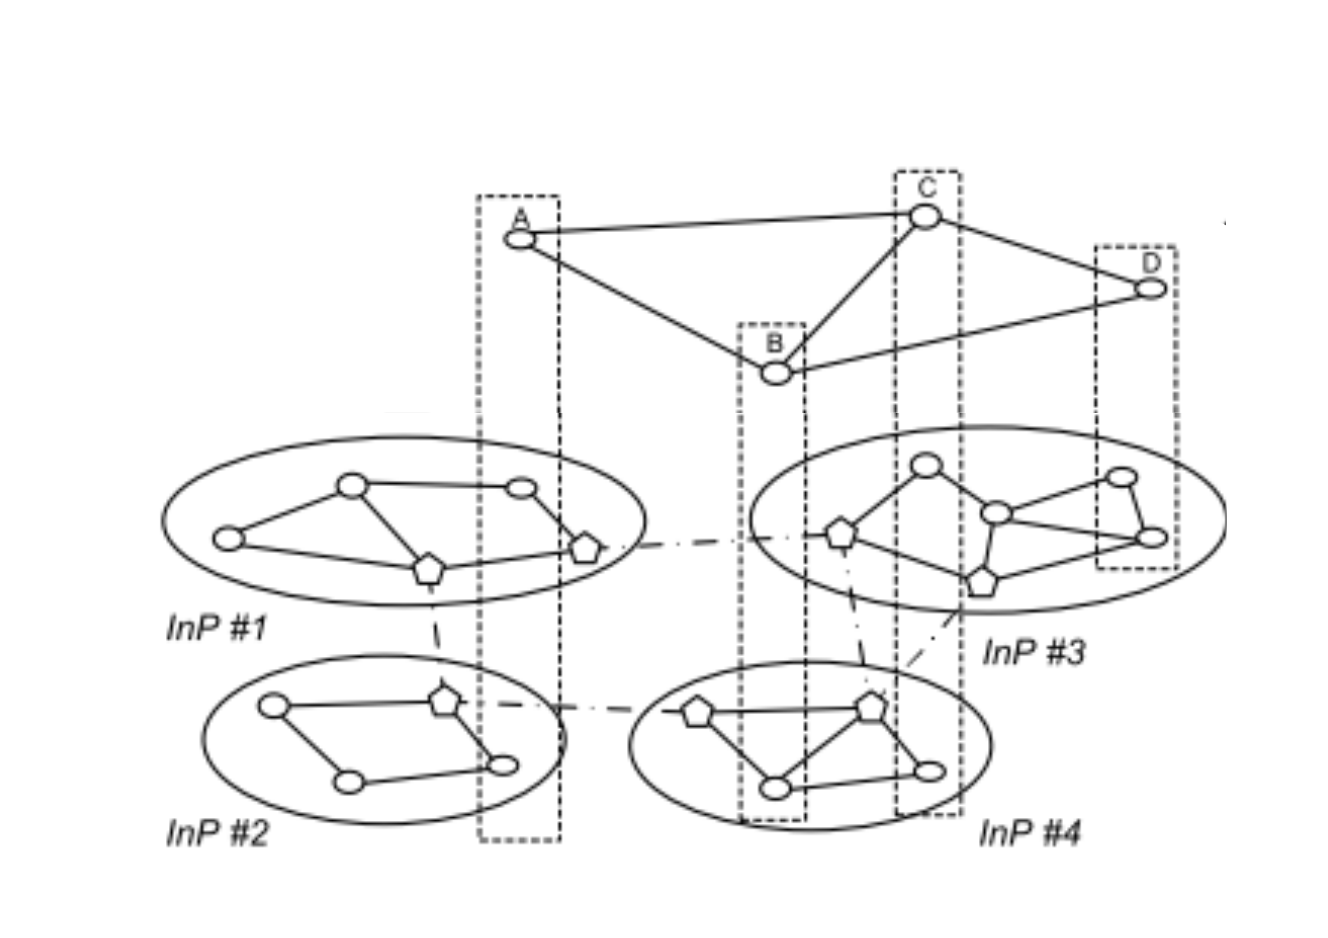
\includegraphics[width=0.5\linewidth]{gfx/multi}    
  	\caption{Multi-provider virtual network embedding \citep{chowdhury2010polyvine}}
  	\label{fig:multi}
\end{figure}

\item Finally, in \citep{zaheer2010multi}, an \textbf{automated service negotiation framework (V-Mart)} is implemented. The V-Mart is also decentralized and based on an auction mechanism, the Vickrey auction model.
Though this approach ensures a fair market, thanks to the Vickrey auction model, it does not guarantee performance. The reason is that the VNE process deployed is a second-stage auction where explicitly all the InPs need to interact during the VN embedding. Thus, the VNE results in a high-demanding task. In addition, the sealed-bid is proposed to be done by a trusted 3rd party, which could cause again confidence issues. Nevertheless, the main V-Mart shortcoming is that it does not solve the LID problem, since it does not enforce inter-domain policies.

\end{itemize}

\section{Analysis of Related Work} \label{analysisOfRelatedWork}

Through relevant examples in supply chain management, as the presented in section \ref{manufacturing}, we can observe the blockchain's potential mainly in areas, where entities are willing to exchange data without trusting a third party. Despite the research does not include detailed specifications, such as the blockchain's type or mining strategy, a useful system design has been provided. In addition, some of the main benefits compared to centralized technologies are contemplated:

\begin{itemize}
	\item \textbf{Disintermediation:} Thanks to the consensus mechanisms, blockchain runs without a central administrator. Thus, intermediaries are not required for realizing transactions which suppresses all the significant costs of involving middle-parties \citep{mainelli2015sharing}. For instance, in the presented example, users were able to transfer ownership, just signing the product's contract.
	\item \textbf{Data management and redundancy:} Blockchain helps us in coordinating, validating and storing the distributed data in a decentralized manner. It also provides automatically redundancy since users own the same data. Reversely, in centralized systems, the users need to explicitly create a backup of the databases, for preventing the loss of data if the system crashes.
	\item \textbf{Unconstrained technology:} As actors can define and establish their own rules (smart contracts), new business models open up.
	\item \textbf{Privacy:} Thanks to cryptography, users can interact with untrusted partners. For example, in the alredy mentioned example, all actors were able to coordinate its services through the PLM process, which before would have been a complex task as they do not trust each other.
    \item \textbf{Transparency and integrity:} All the changes that are made to the contract data are directly visible to the other users. In addition, once a transaction is executed, its immutable since it cannot be altered or deleted.
	
\end{itemize}

On the other hand, in the second part of this chapter, we have investigated related work on multi-provider VNE suffering from LID. A comparison for each of the approaches presented before is shown in Table \ref{tab:Comparison}.

First of all, we can observe that decentralized systems provide obviously a better scalability because the application does not rely on a single point of failure. In centralized systems, this central entity has to be trusted since it stores and manages all the information. In contrast, all the presented related work on decentralized VNE, uses a bidding mechanism to reach an agreement between the SPs and InPs.

Despite being a decentralized system, \cite{zaheer2010multi} uses to some extent a trusted third party (TTP). This is because, it is the only approach offering a sealed-bidding between users, although with the use of a trusted third party. We also notice that in \cite{esposito2013general}, \cite{chowdhury2010polyvine} the bids are exchanged between InPs to cooperate in the VN embedding, which results in undesired computational costs. In contrast, centralized systems \citep{dietrich2015multi}, perform the service negotiation without using auctions, since they trust a middle-party managing these operations.

\begin{table}[bth]
	\myfloatalign \footnotesize
	%18 columns
	\begin{tabularx}{\textwidth}{>{\raggedright\arraybackslash}p{3.5cm} >{\raggedright\arraybackslash}p{1cm}p{0.65cm}p{0.65cm}p{0.65cm}p{0.65cm}p{0.65cm}p{0.65cm}p{0.65cm}p{0.65cm}p{0.65cm}p{0.65cm}p{0.65cm}}
	\textbf{Approach} & \textbf{System} & \rot{\textbf{Scalability}}  & \rot{\textbf{Trusted third party (TTP)}} & \rot{\textbf{Sealed bidding}} & \rot{\textbf{Bid exchange between InPs}} & \rot{\textbf{LID problem solved}} & \rot{\textbf{Location-assisted VNE}} & \rot{\textbf{User notified}} & \rot{\textbf{S-performance}} & \rot{\textbf{L-performance}} & \rot{\textbf{Low VNE cost}} & \rot{\textbf{Low cost (\euro)}}\\ 
		\hline
		Multi-provider VNE framework with VNP \citep{dietrich2015multi} & C & \xmark & \cmark & \xmark & \xmark & \cmark & \cmark & \xmark & \cmark & \xmark & \cmark & \xmark \\ \hline
		CAD - Consensus-based auction for distributed slice embedding \citep{esposito2013general}   &  D & \cmark & \xmark & \xmark & \cmark &  \xmark & \xmark & \xmark & \xmark & \cmark & \xmark & \cmark \\ \hline
		PolyViNE - Policy-based inter-domain VN embedding framework \citep{chowdhury2010polyvine}   &  D & \cmark & \xmark & \xmark & \cmark &  \cmark & \cmark & \cmark & \xmark & \cmark & \cmark & \cmark \\ \hline
		V-mart - Automated service negotiation framework \citep{zaheer2010multi}   &  D & \cmark & * & \cmark & \xmark & \xmark & \xmark & \cmark & \xmark & \xmark & \xmark & \xmark \\
		\hline
	\end{tabularx}
		\caption{Comparison of virtual network embedding approaches - Overview for system features implemented as \textit{yes} (\cmark), \textit{no} (\xmark), \textit{to some extent} (*). Abbreviations: \textit{D} = decentralized, \textit{C} = centralized, \textit{L-performance} = large scenario performance and \textit{S-performance} = small scenario performance.}
	\label{tab:Comparison}
\end{table}

Moreover, one of the main challenges is to solve the limited information disclosure issues. We notice that \citep{dietrich2015multi}, \citep{chowdhury2010polyvine} deal with the problem, accessing public information not considered confidential and performing the VNE under its internal policies respectively. In addition, they provide location-assisted VNE, which facilitate the VN request partitioning across different InPs. The last, it also introduces a notification system, where the InPs gets notified upon VN request, which avoids time spending in request synchronization. 

In general, centralized systems provide a better throughout in small scenarios since all the information is managed by a central entity. Hence, data sharing or user's cooperation is not needed before performing any operation. Conversely, decentralized systems benefit from large scenarios. Firstly, because the more users participating in an auction, the more competitive the market is. Secondly, all the activities are diversified, and thus, the decision-making is more efficient. 

Finally, we classified costs into virtual network embedding and economic. Overall, we observe that VNE costs are lower when using a centralized system \citep{dietrich2015multi}, although when the parties are efficiently coordinated in a decentralized scenario, the costs are also extremely reduced \citep{chowdhury2010polyvine}. Concerning economic costs, they are obviously higher when a centralized system is used, as the application performance depends only on a central entity, which needs to be financed for their computational and maintaining costs.

\section{Summary}

After comparing the different multi-provider VNE approaches exposed throughout this chapter, we find out that each of them introduces innovate features to deal with network virtualization. However, there is no single solution that satisfies at the same time the following requirements:

\begin{itemize}
	\item Scalability.
	\item LID problem approached with data confidentiality.
	\item Large scenarios performance.
	\item Computational and economic low costs.
\end{itemize}

Therefore, the main focus on this thesis will be to investigate and later implement an approach which fulfills the above-mentioned virtual network embedding demands, where we foresee that blockchain could play a significant role.


%*****************************************
\chapter{Design}
\label{ch:design}
%*****************************************

Based on the challenges highlighted in the previous chapter, a conceptional design of a multi-provider virtual network embedding approach using blockchain will be now introduced. First, we define the requirements and assumptions used for the design process. Afterwards, we will present the fundamental goals expected from the system, followed by a general overview of the architecture along with its functionality. In addition, important features for our application will be discussed, in particular, the blockchain type, the mining strategy, the authentication system and the auction model used.

\section{Requirements and Assumptions} \label{requirements}

Since blockchain is a disruptive technology, apparently it seems that it could improve many existing systems. However, is it suddenly blockchain the only way of approaching scalability, security or data handling between organizations? Or why not to use a traditional database rather than a blockchain? The truth of it is that there is not a single solution or better technology than the others, it just depends on user's requirements. Thus, it is important to understand in which scenarios blockchain could replace existing infrastructures. For this purpose, in Figure \ref{fig:bcFlowchart} we present a flowchart \citep{wust2017you}, which pretends to guide users in determining whether blockchain is the appropriate solution to resolve their problems, and if yes, the suitable BC type. We will also follow the diagram to decide if our defined VNE scenario demands match the blockchain use case.

\begin{figure}[bth]
	\centering
	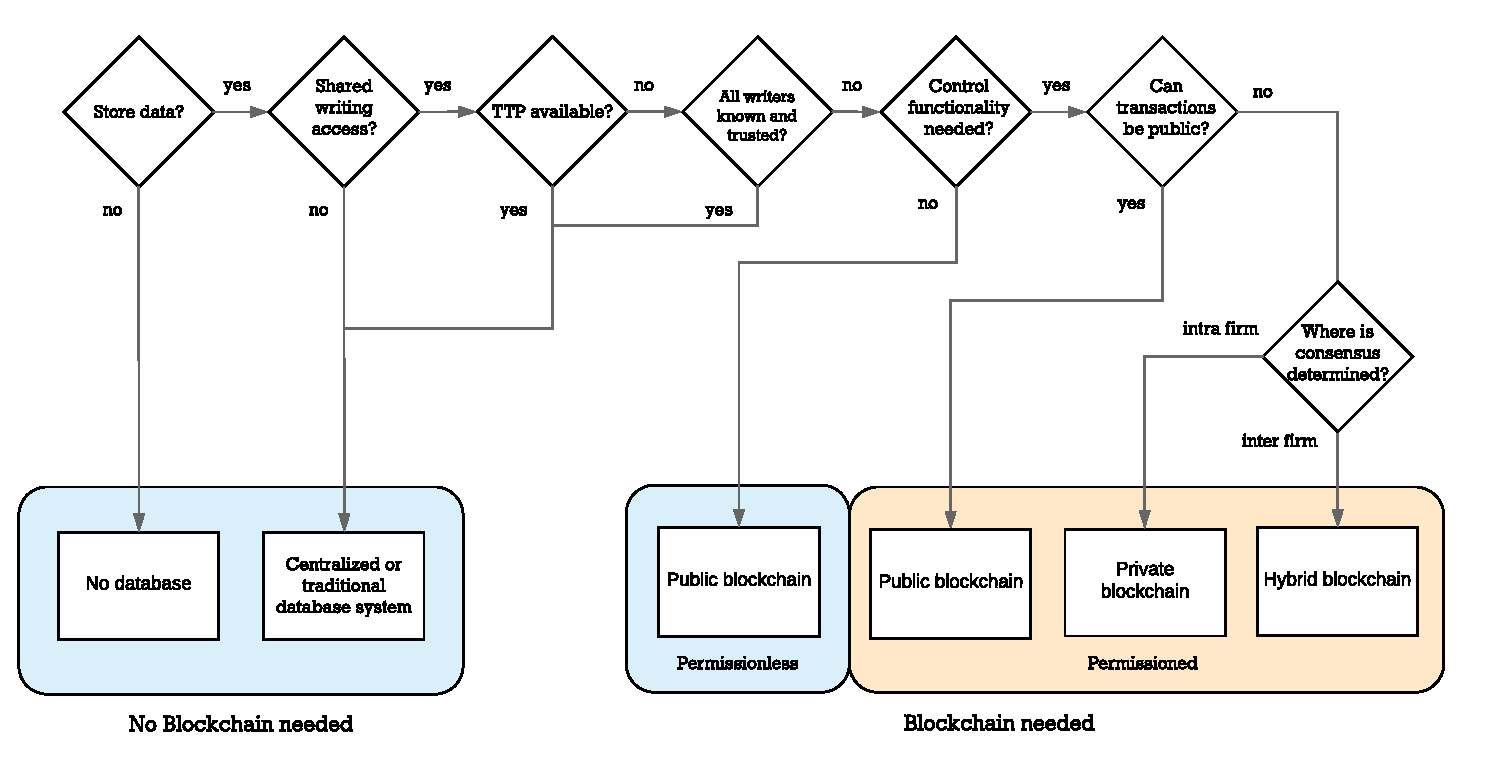
\includegraphics[width=1\linewidth]{gfx/bcFlowchart}    
  	\caption{Flowchart to determine whether blockchain is the suitable solution. Adapted from \citep{wust2017you}}
  	\label{fig:bcFlowchart}
\end{figure}

Before starting with the flowchart, one statement needs to be clear: if the user does not need to store data, no blockchain or database is required. The discussion arises when multiple writers want to exchange data without relying on a trusted third party (TTP). In this context, a writer is a user that performs the four basic functions of persistent storage: create, read, update and delete data (CRUD). If they trust a TTP, a traditional or centralized database will always provide a better throughput. However, if this is not the case, then the user should first consider if all the writers are known and trusted. If so, again a typical database (e.g. SQL) will be better positioned. If all the last requirements are satisfied, or in other words, multiple untrusted writers are willing to update the state of a system without trusting a middle actor, it is then that using a blockchain is a reasonable solution.

In Figure \ref{fig:bcFlowchart}, we also classify blockchains into two groups: \textit{permissionless} and \textit{permissioned} blockchains. To decide between these two approaches, the user should consider if he is willing to control his customized blockchain, creating his own specifications. For example, the main network of Bitcoin and Ethereum is permissionless, where users are added to the network and thus, restricted to its policies. In Table \ref{tab:blockchainTypes} the main characteristics of each blockchain type are summarized. Scalability is an important topic in the blockchain domain, where we distinguish: node scalability and performance scalability. The former is the capacity to add new participants in the blockchain without losing performance, and the latter is the number of transactions executed per second. In addition, note that some features depend on the blockchain design decisions since permissioned blockchains capabilities are easily modifiable. For example, if consensus algorithms are used, the interaction between users should have a cost in order to ensure performance, i.e miners need to be rewarded with transaction fees.

\begin{table}[bth]
	\myfloatalign \footnotesize
	%18 columns
	\begin{tabularx}{\textwidth}{>{\raggedright\arraybackslash}p{4cm} >{\raggedright\arraybackslash}p{6cm}>{\raggedright\arraybackslash}p{6cm}}
	\textbf{Features} & \textbf{Permissionless} & \textbf{Permissioned}\\ 
		\hline
		Type & Public & Public, private and hybrid blockchain \\
		Control functionality/ Transaction processing & Fully decentralized & One or a small group of pre-selected entities \\
		Access control & Open access & Authorized access \\ 
		Number of users & High & Low \\
		Number of untrusted users & High & Low \\
		Writers & Any user participating & Permissioned group of people, e.g. bank customers\\
		Centrally managed & No & (*) \\
		Security & Consensus algorithms (e.g PoW) & (*) \\
		Transaction fee & Yes & No (*) \\
		Trusted & No & Yes \\
		Node scalability & High & Low \\
		Performance scalability & Low & High \\
		Use cases & Cryptocurrencies (e.g. Bitcoin) & Transactions in business networks (Hyperledger Fabric) \\ \hline
	\end{tabularx}
		\caption{Types of blockchain: permissionless vs permissioned. Adapted from \citep{wust2017you}. (*) states for depending on blockchain design decisions.}
	\label{tab:blockchainTypes}
\end{table}

Furthermore, as stated in Figure \ref{fig:bcFlowchart}, permissioned blockchains are divided into:

\begin{itemize}
	\item \textbf{Public permissioned blockchain:} Decentralized, all the participating users are allowed to read the system's state (transactions can be publicly verified), but just some of them have writing privileges.
	\item \textbf{Private blockchain:} Centralized, with access and writing permissions restricted to a set of users. Note that in the flowchart this corresponds to an intra-firm consensus since it is only managed by a single organization. We understand by firm a traditional company or a pre-selected group of users.
	\item \textbf{Hybrid/Consortium blockchain:} Partly decentralized, the blockchain management is controlled by a pre-established set of entities (inter-firm). In this model, each of the firms typically possesses a blockchain node to coordinate and ensure the system's functionality. Note that compared to the private blockchain, multiple firms maintain and serve the infrastructure rather than a single one. Thus, a consensus between these parties is also extremely needed. For example, currently, several banks deploy common blockchains to manage their shared data and reduce intermediaries costs. In this case, each bank will control a node, resulting in a better throughput in terms of scalability.
\end{itemize}

After presenting the blockchain use cases and types, we observe some similarities between a traditional shared database and a permissioned private chain, since they are both managed by a group of users, which simultaneously maintain the same confidential data. Despite private blockchains could be seen only as another term used to name shared databases, the truth of it is that each technology has its trade-offs, without mentioning scalability or cost issues. On one hand, centralized databases will always have better throughputs since, in addition to the basic transaction operations, blockchains need to perform cryptographic verifications, and ensure a consensus between the other participating nodes. On the other hand, private blockchains are less prone to malicious attacks, inasmuch as they spend a longer period in checking errors or validating transactions, than regular databases. The blockchain also organizes data into blocks, which is updated only appending new data. Therefore, as already noted, if users trust each other and a high-performance is desired, using a blockchain will not be the suitable solution.

\subsection{Virtual Network Embedding with LID scenario}

In section \ref{analysisOfRelatedWork}, we have concluded that although excellent research in network virtualization have been conducted, to the best of our knowledge, there is still not an approach solving the LID problem in terms of scalability, confidentiality, and low-cost performance. Thus, after having spotted the main benefits of integrating blockchain in real-scenarios, among which disintermediation, privacy  and transparency need to be highlighted, we assume that this technology could improve the VNE business process. Nevertheless, first, we should investigate whether our scenario could be integrated in a blockchain.

In network virtualization, we mainly encounter users with two different roles: Infrastructure Providers and Service Providers. Moreover, as the VNE is typically performed by the same parties across the countries, e.g. Deutsche Telekom, Vodafone or O2 in Germany, the scenario is restricted to a limited amount of users that barely changes. Therefore, we are facing an application where multiple known users but probably not trusted, want to reach a virtual network agreement, without relying on a third party. The decision of not including a TTP or VNP is mainly to avoid exchanging the InPs internal network cost models to an intermediate actor.

Observing the last mentioned requirements, we foresee that blockchain could be a suitable solution for our VNE scenario suffering from LID. However, the significant choice between blockchain types still needs to be argued. Obviously, the service negotiation between InPs and SPs is performed in a private environment, which automatically removes the permissionless and permissioned public blockchain options. Hence, the decision should be taken between a private or a hybrid blockchain.

One of the main requirements noticed from the previous related work is that our approach must not suffer from scalability issues. Accordingly, using a private blockchain, which is a centralized system managed by a single firm, will provoke that users rely again on a central point or trusted party, converting it to an unfeasible workaround. Thereby, the \textbf{partly decentralized hybrid blockchain} seems to be the most suitable solution. In this scenario, a firm corresponds to each interested InP or SP willing to possess and control a blockchain node, in order to ensure the network virtualization functionality.


\subsection{Smart Contracts and Ethereum}

After having spotted the most suitable blockchain type for our VNE environment, the non-trivial decision of selecting a blockchain platform needs to be taken. Prior to this, we need to consider whether our scenario could profit from the potential of smart contracts. Despite in subsection \ref{smartContracts}, it has been discussed what smart contracts are, it is also required to notice when they can be used. Thereupon, due to its extended dimension, a market study regarding smart contracts and its application fields will not be conducted. Nonetheless, we will enumerate the main usage examples of smart contracts in business to business processes \citep{blockchainBerkeley}:

\begin{itemize}
	\item \textbf{Settlement agreement:} Since smart contracts can be personalized, it enables that participants can reach any kind of agreement without involving third-parties costs.
	\item \textbf{Frequently executed tasks:} Users regularly performing the same operations, can accelerate this process by depicting them on a smart contract code.
	\item \textbf{Self-operating databases:} Thanks to the blockchain, secured shared databases with low-costs are easily deployed. In addition, smart contracts can automate the interaction with this stored data, providing speed, real-time transparency and at the same time, opening new business models. 
\end{itemize}

In the presented network virtualization example, as the users negotiate the lease of virtual nodes over and over to reach an agreement, this task could be perfectly reflected in a contract code. Apart from dealing with smart contracts, as later we will implement a prototype, the blockchain platform chosen needs to fulfill the following prerequisites \citep{macdonald2017}: 

\begin{itemize}
    \item \textbf{Easy to build, use and learn:} A low effort in setting the platform is essential. Thus, the smart contracts should be written or derived from common languages in the world of programming, such as JavaScript or Python.
    \item \textbf{Support and documentation:} A consolidated platform, which is not in its early stages and with a high-maturity level achieved, is extremely needed. An active community of developers behind the project is also fundamental, e.g. with a considerable number of Github\footnote{\url{https://github.com/}} stars and forks.
    \item \textbf{Blockhain type:} Though it could be desirable that the main network is permissioned and hybrid or private, currently, in open source code platforms, the blockchain types can be modified. Thus, that the predefined main network type matches the desired one, is not a must-have feature.
\end{itemize}

\begin{table}[bth]
	\myfloatalign \footnotesize
	%18 columns
	\begin{tabularx}{\textwidth}{>{\raggedright\arraybackslash}p{2.5cm}>{\raggedright\arraybackslash}p{2.5cm}>{\raggedright\arraybackslash}p{2.5cm}>{\raggedright\arraybackslash}p{2.5cm}>{\raggedright\arraybackslash}p{2.5cm}>{\raggedright\arraybackslash}p{2.5cm}}
		\textbf{Characteristics} & \textbf{Bitcoin} & \textbf{Ripple} & \textbf{Ethereum} & \textbf{Hyperledger Fabric} & \textbf{R3 Corda}\\ 
		\hline
		\textbf{Application} & Payments & Payments & General purpose & General purpose & Financial services \\
		\textbf{Governance} & Bitcoin developers & Ripple Labs & Ethereum developers & Linux Foundation & R3 \\
		\textbf{Main network} & Permissionless, public & Permissioned, public & Permissionless, public and private & Permissioned, private and hybrid & Permissioned, private and hybrid \\
		\textbf{Data model} & UTXO-based & UTXO-based & Account-based & Account-based & UTXO-based \\
		\textbf{Configuration effort} & Low & Low & Low & High & High \\
		\textbf{Support and Documentation} & High & Medium & High & Medium & Low \\
		\textbf{Smart contract language} & - & - & Solidity (JS), Serpent (Python) and LLL & Go, Java & Kotlin, Java \\
		\textbf{Currency} & BTC & XRP & ETH & None & None \\
	\hline
	\end{tabularx}
		\caption{Comparison of different blockchains platforms. UTXO stands for Unspent Transaction Outputs.}
	\label{tab:blockchainComparison}
\end{table}

In table \ref{tab:blockchainComparison}, a comparison of the most common blockchain platforms, in our opinion, is depicted. Since in our application a scripting language with smart contracts is preferrable, and Bitcoin and Ripple by default do not incorporate them, these platforms are automatically discarded. On the other hand, Hyperledger Fabric and R3 Corda are popular used platforms, whose main network perfectly fits our requirements. However, they provide customized blockchains with a high configuration effort, since its specifications need to be carefully designed. Thus, as a platform with a straightforward setup and usage is required, Ethereum seems to be the better positioned.

Ethereum is a mature and easy to build project based on smart contracts with a large number of developers behind, who are actively discussing and improving its functionality. Thanks to this, the creation of new business models is extremelly facilitated for newcomers. Furthermore, Ethereum smart contracts are written in Solidity and Serpent, which are similar to JavaScript and Python respectively. Among these, Solidity seems to be more consolidated, which at the same time better matches our programming languages knowledge. Despite the fact that Ethereum's main network (public permissionless), is not the ideal for our scenario (permissioned and hybrid), the simple and easy set up of the platform's environment, will allow us to quickly deal with these issues. The last but not least, Ethereum Virtual Machine (EVM) is a Turing-complete system, which helps us in obtaining the maximum benefit from the smart contract's potential.

On balance, thanks to the blockchain, more precisely Ethereum and smart contracts, the untrustworthy VNP could be replaced with a secure, flexible and coordinated end-system. In this scenario, the reliance will now be distributed among multiple blockchain nodes rather than just on a costly single entity. However, challenges, such as the scalability or the service negotiation performance, will have to be thoroughly investigated along the thesis.

\section{System Design}

Based on the requirements and assumptions defined in the previous section, the design of a multi-provider virtual network embedding scenario using the blockchain technology is now presented. The system's design considerations are described in the following manner. At first, the fundamental goals expected from the system are defined, followed by a general overview of the architecture and later on, the essential design features are also discussed.

\subsection{Fundamental Goals}

In general, the fundamental goals for network virtualization relies on simulating hardware networks, providing improvements in terms of flexibility, manageability, and costs. In this scenario, the SPs are willing to embed virtual nodes across different InPs to create customized virtual networks. This embedding task consists first in the VN request partitioning and later, in the corresponding mapping to the InP's physical nodes, such that virtual node and link requirements are fulfilled. However, the problem appears when InPs are not willing to disclose detailed information about their resources availability or network topologies, which is indispensable for the VN partitioning efficiency. In this thesis, the VN partitioning is treated as a cost minimization problem, where the service provider pursues the minimum VN embedding cost. In a real scenario, there are other parameters that could be taken into consideration, such as quality of the service or the proportioned capacity, although they will not be the focus of this paper.

In a multi-provider scenario with full information disclosure (Figure \ref{fig:problem}.a), since the infrastructure provider's internal information is publicly available, the VN request partitioning is efficiently computed. Conversely, the lack of data in a limited information disclosure scenario (Figure \ref{fig:problem}.b), directly affects the VNE throughput. Nevertheless, there is some information not considered confidential by the InPs, such as the virtual node type cost or the InPs peering nodes. For instance, in Figure \ref{fig:problem}.b, InP2 has two peering nodes with virtual node type $\{A,B,D,E\}$ and $\{F,G\}$ respectively. Thus, in this thesis, new strategies and approaches to facilitate the service negotiation process between the InPs and SPs, must be developed. 

Moreover, in section \ref{analysisOfRelatedWork}, it has been contemplated that decentralized approaches tend to use auctions to negotiate the network workflows. Regardless of the auction model applied for our VNE framework, there are several objective metrics that must be considered: 

\begin{itemize}
    \item \textbf{Efficient:} The virtual network embedding must be efficient in terms of synchronization, communication, and data sharing between the participating users.
    \item \textbf{Equality:} All participants, namely service providers and infrastructure providers, must have the same role's privileges. In other words, all SPs must be able to request the same amount of virtual networks over time and InPs bids must be treated equally in the application.
    \item \textbf{Market fairness:} The auction model requires that the SPs find the desired service at the lowest price and that the InPs obtain the highest possible revenue for the offered service.
    \item \textbf{Data confidentiality:} At the moment of bidding, the bids should be kept in secrecy in order to not alter the auction progress. In the end, the winners can be publicly known.
    \item \textbf{No trusted auctioneer:} Since confidentiality is required, a middle party or auctioneer should not be capable of managing the auction workflow and thus, accessing the private bidding values.
     \item \textbf{Automated:} The virtual network embedding process needs to be automated with a friendly and easy-to-use framework, which guides the users through their operations. 
\end{itemize}

\begin{figure}[bth]
	\centering
	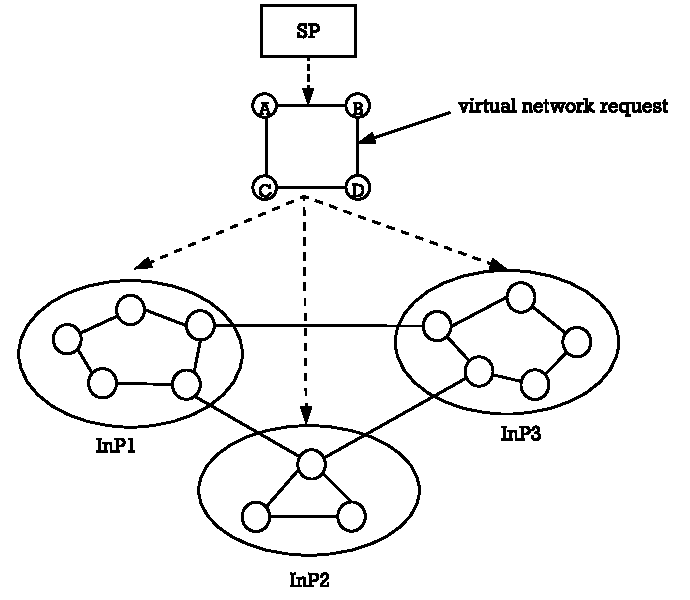
\includegraphics[width=1\linewidth]{gfx/Problem}    
  	\caption{Substrate network visibility. (a) Full information disclosure (FID). (b) Limited Information Disclosure (LID). Adapted from \citep{dietrich2015multi}}
  	\label{fig:problem}
\end{figure}

\subsection{System Architecture}

\begin{figure}[bth]
	\centering
	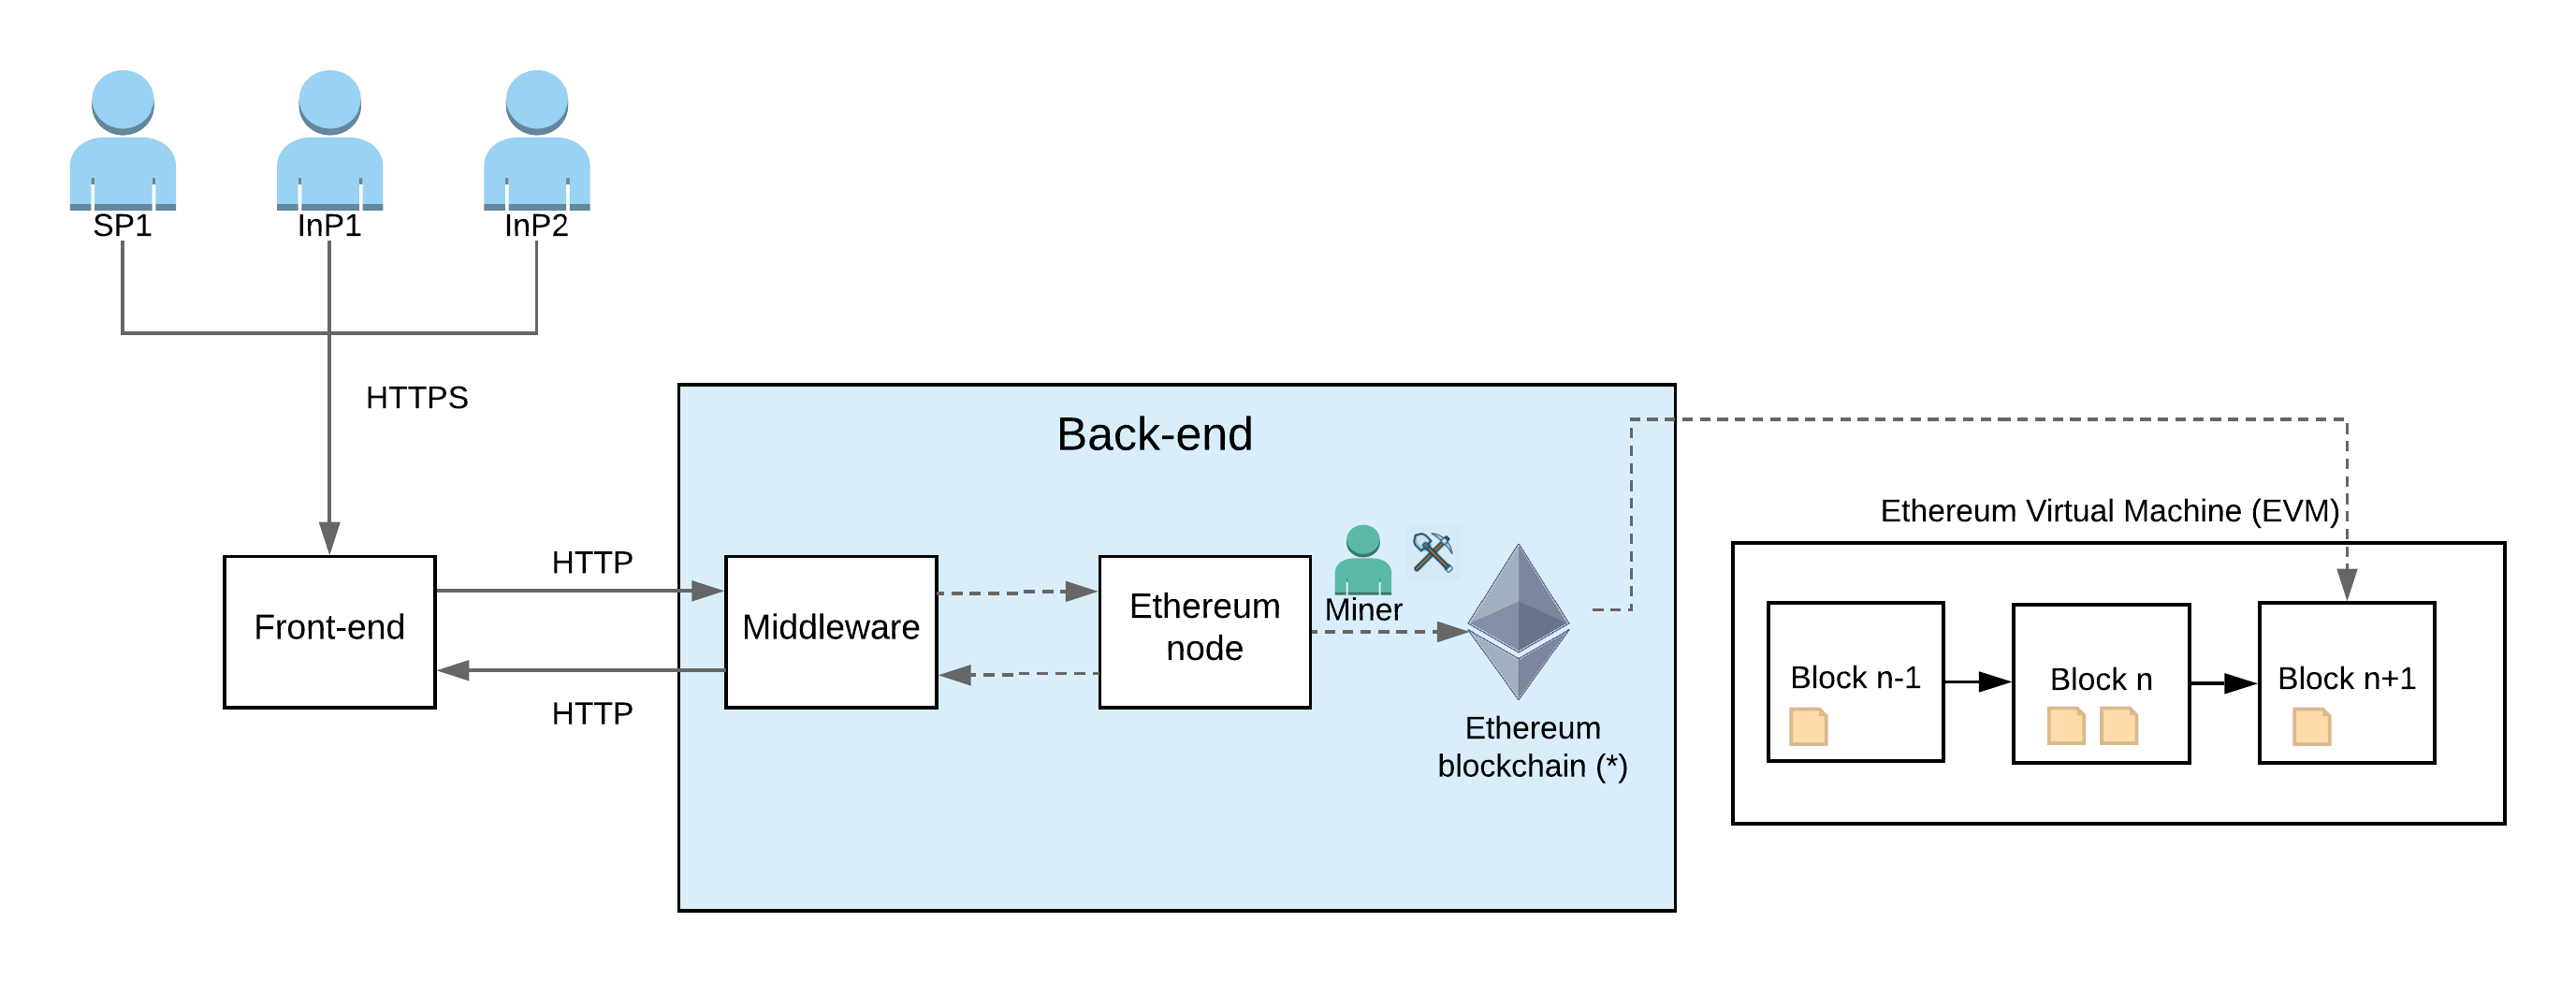
\includegraphics[width=1\linewidth]{gfx/designWorkflow}    
  	\caption{Design system architecture. UP states for upper bound cost and L for location}
  	\label{fig:designWorkflow}
\end{figure}

After defining the main VNE problem that needs to be addressed, and describing the goals and metrics required for the design of our scenario, a system architecture is now presented, see Figure \ref{fig:designWorkflow}. Firstly, the proposed design shows the main components of the system, which are:

\begin{itemize}
    \item \textbf{Private group of users:} The system is composed of a private group, in which participants can be infrastructure providers or service providers. Since in private groups only certain members are allowed to access and alter the data, in this design, new users must ask for permission before joining the network. Furthermore, once entering the group, the newcomer can optionally act as a miner or just use the application without the need of maintaining a blockchain node.
	\item \textbf{User interface (UI):} Through a friendly user interface,  each member will efficiently interact with the blockchain application. Depending on the user's role, i.e infrastructure providers or service providers, the UI will provide different functionalities. For example, SPs have the ability to request virtual networks and InPs to bid for the proposed virtual nodes, but not the other way around. Thus, the available operations must be restricted to the user's privileges.
	\item \textbf{Ethereum blockchain:} One of the main differences between the Bitcoin and the Ethereum blockchain is that they are transaction-based and account-based respectively. For this reason, apart from a list of transactions, each Ethereum's block also stores the most recent state, i.e. the current accounts list with the corresponding balances. Nevertheless, every blockchain starts with the block 0, also called \textit{Genesis block}. Since it is the first block, is the only one not pointing to a predecessor and it is typically hardcoded in a file called \textit{genesis.json}. This file contains some of the blockchain specifications, such as the difficulty or the gas limit. By modifying the value of these parameters, users are allowed to create blockchains based on their requirements. More details about the genesis file content used in our system will be discussed in chapter \ref{ch:implementation}.
	\item \textbf{Smart contracts:} In the previous point, we have mentioned that each Ethereum block stores a list of accounts with their corresponding balances, among others. These accounts can be externally owned accounts (users) or contract accounts (smart contracts). Our focus will be on the last since they enable reflecting user's needs into code. These smart contracts can be created or called either from another contract or simply by an EOA. In our system's design, the first block contains two fundamental static contracts, whose address will be user-known and hence, permanently requestable. On one side, the \textbf{Users} contract will store all the participant's information, and whenever a new user registers, this contract's data will be modified. On the other side, the \textbf{Auctions} contract will be the broker used for starting an auction, which creates a new contract with the requested data.

\end{itemize}

To provide a clearer view of the last mentioned components, the application's functionality needs to be introduced. This VNE process entails the following steps (Figure \ref{fig:designWorkflow}):

\begin{enumerate}
    \item \textbf{VN request:} A service provider requests a virtual network by calling the \textit{Auctions} contract address, e.g. 0x452c812a1... The request can be represented in a graph as $G_k = (N_k , d_{ij})$ where $N_k$ consists of a set of virtual nodes, represented by $\{A,B,C,D\}$ and $d_{ij}$ as the bandwidth demand between the virtual nodes $i,j \in N_k$. Each $N_k$ is formed by a collection of attributes, such as the desired location $l_k$ or the upper bound cost $u_k$. In case an upper bound cost for the whole network is specified $u_{G_k}$, each virtual node $u_k$ will be averaged $u_k = \frac{u_{G_k}}{k}$
    \item \textbf{Resource matching:} Once the \textit{Auctions} contract is called, it will first check the associated set of attributes (e.g. location) of the requested virtual nodes. These parameters will be used to match the corresponding InPs from the \textit{Users} contract. For instance, virtual nodes $\{A,B\}$ and $\{C,D\}$ will be matched with InPs possessing physical nodes in Germany (DE) and Switzerland (CH) respectively. In case no location is specified, the VN request will be broadcasted to all the registered infrastructure providers.
	\item \textbf{Auction start:} Using the previous information, the corresponding smart contract, i.e. \textit{limited time auction}, is automatically created. This contract contains: (i) the data related to the virtual network nodes and links, (ii) the address of the SP willing to lease virtual nodes, (iii) a list of all the InPs addresses matched and (iv) an \textit{end-time} field. Since the bidding cannot last forever, in the first step, the SP must also add this \textit{end-time} field to the request.
 	\item \textbf{Notification and bidding period:} After the new auction contract creation, the included InPs, which are the only users with the ability to bid for the resources, are notified. Despite having a full view of the VN request and knowing the other matched InPs, each InP is only allowed to bid for their paired resources. For instance, InPs from Germany can only bid for the resources $\{A,B\}$. Before bidding, these users typically evaluate the proposed virtual nodes into their substrate network, depicted as $G_s = (N_s , L_{ij})$, where $N_s$ are the physical nodes and $L_s$ the physical links between the $N_s$ nodes. Although InP's goal is to allocate the maximum amount of virtual nodes at a reasonable cost, a single InP can barely serve all the virtual nodes requirements. As a result, the virtual network will be supplied by different infrastructure providers. More details about the bidding mechanism will be presented in section \ref{vickrey}.
 	\item \textbf{VN request partitioning and mapping:} Once the auction has finished, each virtual node will be assigned to the winning InPs so that the VN embedding cost is minimized (\textbf{min-C}). These winners will be publicly known by all the other participating users and thereupon, the service provider will contact them to ultimate the VN setting up, i.e. to perform the VN segment mapping.
\end{enumerate}

In a nutshell, the presented system design uses the blockchain technology, in particular, smart contracts, to enhance the VN partitioning efficiency in a multi-provider scenario with limited information disclosure. Nevertheless, up to now, this is only a conceptual design with a lot of features that must be further discussed.

\subsection{Blockchain Type and Mining Strategy}

Ethereum's main network, as Bitcoin, is public and permissionless, where all the users have access to the transferred values between accounts. However, since our described scenario has a small number of users, the fully decentralized approach will directly affect the application performance. Thus, as concluded in section \ref{requirements}, our focus is on \textbf{permissioned hybrid blockchains}, where a set of inter-firm entities control and maintain the blockchain functionality. 

On the other hand, the default Ethereum's consensus algorithm will be used, which is at the time of writing, the \textbf{Proof-of-Work} protocol. Nevertheless, since the blockchain can be customized, in chapter \ref{ch:implementation}, other mining strategies will be further in investigated.

In summary, although the Ethereum's main network is public and permissionless, it can run as a private or hybrid blockchain, with the technology mechanisms and protocols remaining unaltered.

\subsection{Authentication System} \label{authenticationSystem}

In the following, we will discuss how a user is registered and authenticated to the system, see Figure \ref{fig:authenticationDesign}.

First of all, in order to deploy and use the presented design, one user needs to set up the environment. Afterwards, he can invite others users to join his network, i.e. to create an Ethereum account (EOA) for the application. However, once these users are registered, the communication must be secured. For this reason, the blockchain technology uses the \textbf{public-key cryptography}, also called asymmetrical cryptography. In particular, Ethereum uses the \textit{Elliptic Curve Digital Signature Algorithm (ECDSA)} to validate the origin and integrity of messages. 

\begin{figure}[bth]
	\centering
	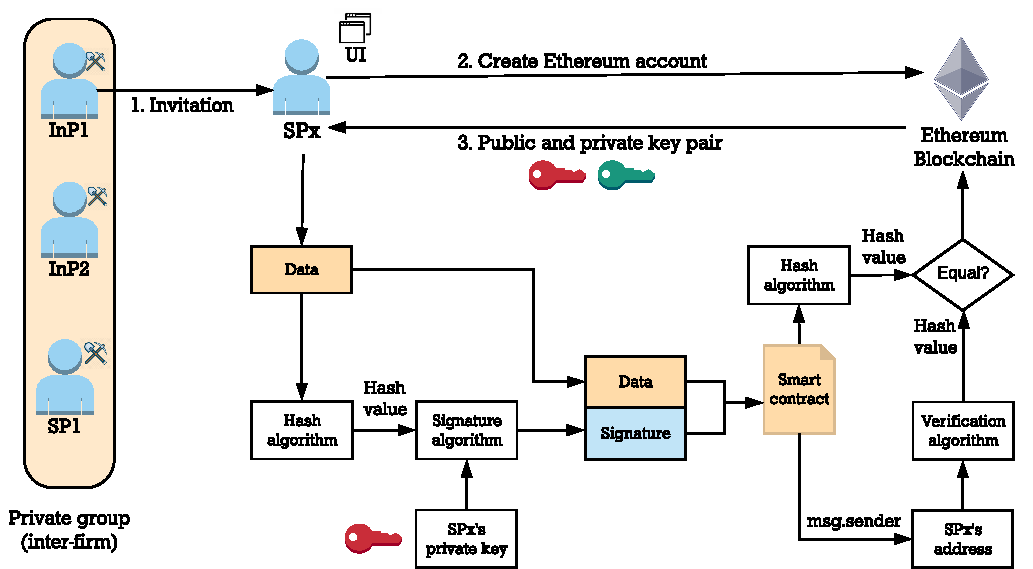
\includegraphics[width=0.9\linewidth]{gfx/authentication_design}    
  	\caption{Authentication design and public-key cryptography}
  	\label{fig:authenticationDesign}
\end{figure}

In addition, the Ethereum address is also extracted from this key pair, more specifically, from the last 160 bits of the \textit{SHA3-256}\footnote{\url{https://en.wikipedia.org/wiki/SHA-3}} hash of the public key. Thus, once a user creates a new Ethereum account, the blockchain generates a random public and private key pair. Since the private key can be used by an attacker to access the ledger or to impersonate the account's owner, it is essential to keep it secure.

Furthermore, users must always digitally sign their operations to ensure authenticity and integrity, by providing a \textbf{digital signature}. In this process, they will use the private key to produce a short string of the data, called signature. In this way, the receiver can verify that the data has been signed by who claims to be the owner and that the content has not been altered.

On the other hand, it is important to note that smart contracts, if well-defined, they also provide security in terms of access control and confidentiality. Despite the fact that Ethereum users can create and own smart contracts, its content is not always accessible or alterable. For instance, when users are not willing to broadcast the contract's information or simply when they want to avoid that every party can alter the state of the contract. Thus, these operations are restricted only to a set of users, whose addresses need to be known by the contract account. In our VNE scenario, the matched InPs are the only users allowed to bid on specific resources.

Therefore, although the blockchain is a decentralized and distributed technology, where the actors do not know or trust each other, thanks to cryptography, a secure communication between all the participants is achieved. In addition, since Ethereum uses smart contracts, the data access can also be restricted and with its content hardly manipulated.

\subsection{The Vickrey Auction Model} \label{vickrey}

In section \ref{auctionMechanisms}, after judging different auction types, it is concluded that a \textbf{one-sided reverse Vickrey auction} seems to be the most suitable for network virtualization. In the following, a more thorough examination in adapting this auction model in the multi-provider VNE scenario suffering from LID will be presented.

In this case, our auction procedure will start with the SP requesting a virtual network along with an upper bound, the last being the maximum amount of money the SP is willing to pay. Then, the InPs will estimate the request requirements (e.g: nodes availability or costs) in their infrastructure and thereafter submit their bids. In other words, the InPs will be sellers submitting bids and SPs the consumers requesting a service.

Thus we arrive at the one-sided sealed Vickrey auction
model for V-Mart. Each VN Bidder receives a RFQ from the SP and submits a per virtual resource price quote for each resource it is willing to host. We will discuss how this per resource price quote can be determined later in this section. The SP takes all the quotes for each virtual resource and modifies the quote of each VN bidder to the quote of the
immediate


\begin{figure}[bth]
	\centering
	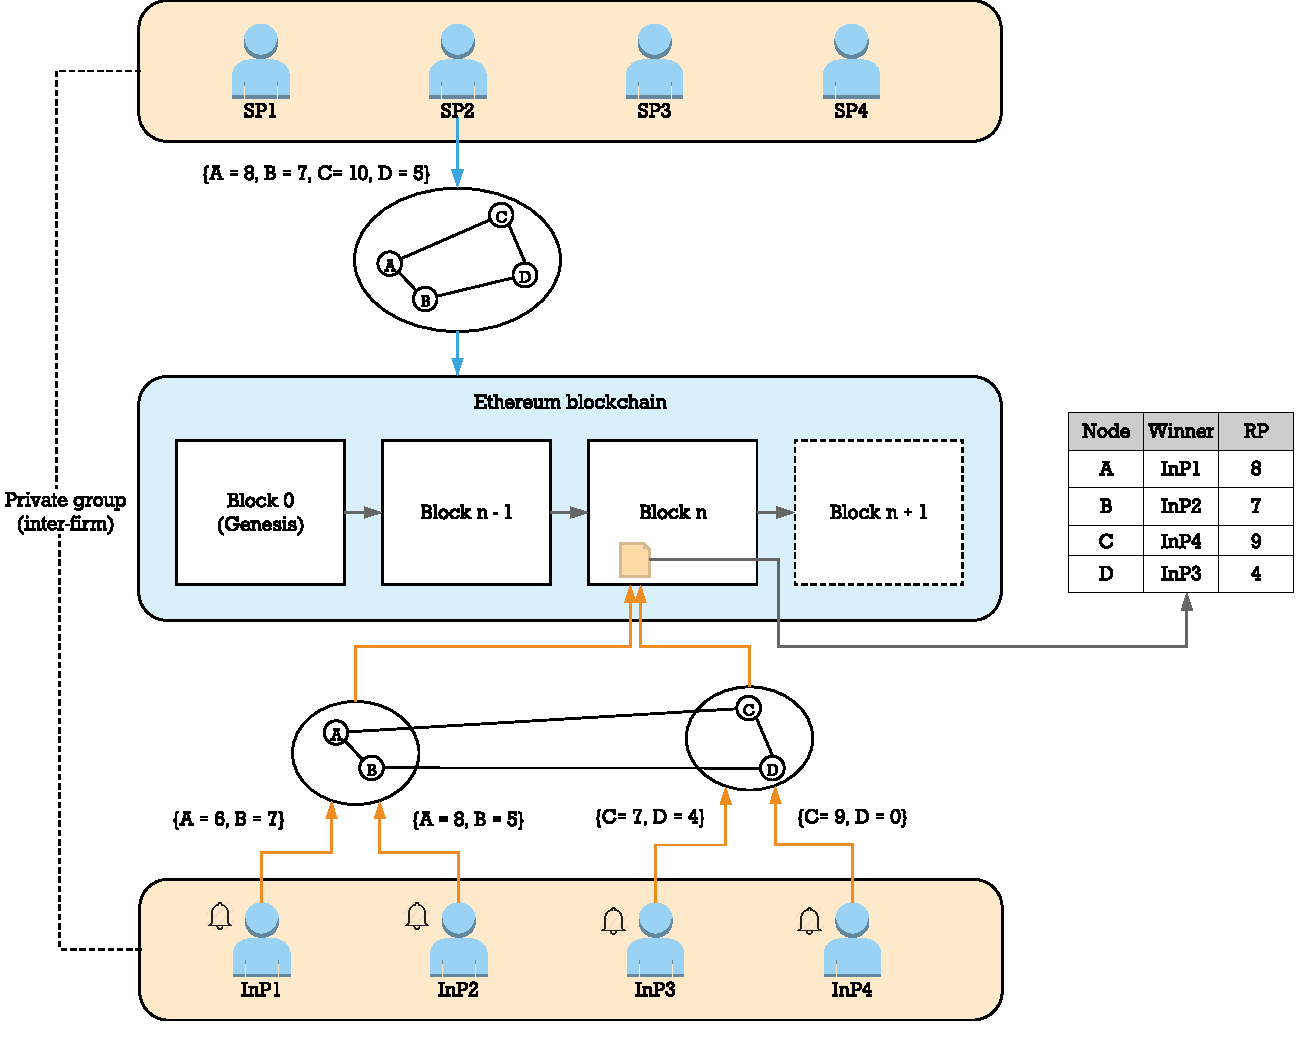
\includegraphics[width=0.9\linewidth]{gfx/vickrey}    
  	\caption{Vickrey auction}
  	\label{fig:vickreyAuction}
\end{figure}

WHY AND WHAT IS + PROCESS PICTURE EXPLANATION
ATTACKS COUNTERMEASURES \citep{boyd2000security}
MULTIPLE ITEMS AUCTION \citep{ausubel2006lovely}
WHO OPENS THE BID? (PAPER EXPLANATION) \citep{ausubel2006lovely}
CONS
SOL
Due to the lack of detailed knowledge of the substrate topologies, we will not be in position to account for all intra-provider link costs (COPIED).
For VN request partitioning, we seek the assignment of the requested virtual nodes to the disclosed peering nodes, i.e.,NvP, such that the cost for the SP isminimized (COPIED)


It is important to note that in our scenario, similar to \citep{zaheer2010multi}, the \textbf{lowest auction} will win and not the highest. The reason is that at the end the SPs is who will pay the bid value. For instance, suppose that all the InPs make an offer close to the upper bound specified by the SP. If the highest bid wins, the SPs will always end-up paying approximately its upper bound (unfair). However, if the lowest bid wins, the system ensures that the InPs submits a bid proportional to the real cost since it will be the minimum amount of money that they could earn.

However, the second-price concept needs to be thoroughly investigated as long as a bidder can submit multiple bids. Imagine an scenario, where a single bidder A submits two bids: \{1 \euro,9 \euro\} for a service with a real cost 5 \euro. In this case, this buyer will end up paying 1 for the service. Therefore, the second-price auction model needs always to be compared between bidders and not between bids. Suppose the last example, with a second bidder B submitting \{5 \euro, 6 \euro\}. At the end user A, will win the bid but paying 6 \euro, risking that if he would have been the only user bidding, he would have payed 9 \euro.

Explain that an auction could use a multi-dimensional process (more parameters).

Package pricing or volume discount?

What can be externally extracted from a contract? Since value transfers cannot be blinded in Ethereum, anyone can see the value and therefore the highestBid. Sol: We can just see the address. That's a problem if there are just a few users. Do research on amount of users needed to solve the problem.

\section{Summary}

During this paper, the Ethereum blockchain will be used to perform a service negotiation (Vickrey auction) and later to track its possession throughout the supply chain process. This will be exemplified by a web application implementation, focused on network slicing. Thus, blockchain strengths and weaknesses will be further investigated.

The blockchain technology, in particular, secure smart contracts on the Ethereum platform, will be used to approach a real-world scenario. A decentralized application (third category) that enhances supply chain performance, will be implemented. More precisely, network virtualization providers and customers will improve its communication, through the use of a web application (front-end) connected to the blockchain (back-end).

We do not claim that our approach is the best or the only way
of performing VN embedding. On the contrary, it is more an add-on feature that can be merged with most of the existing solutions. In this scenario, the main goals are to remove the middleware or virtual network provider, by using a new prominent technology such as blockchain. Thus, a new decentralized, automated and secure system between the SPs and InPs will be created, which benefits from the blockchain potentials. Furthermore, to the best of our knowledge, this is the first approach using blockchain in the network virtualization context, and thanks to smart contract's flexibility, it can serve as a starting point for upcoming investigations.

%*****************************************
\chapter{Implementation}
\label{ch:implementation}
%*****************************************

\hint{This chapter should describe the details of the implementation addressing the following questions: \\ \\
1. What are the design decisions made? \\
2. What is the environment the approach is developed in? \\
3. How are components mapped to classes of the source code? \\
4. How do the components interact with each other?  \\
5. What are limitations of the implementation? \\ \\
The section should have a length of about five pages.}

1. How a contract is compiled in to the Ethereum BC.
2. Technologies used (GETH vs ETH NW, web3, Solidity, truffle).
(The Genesis block is the first block in a blockchain. It is always hardcoded in the blockchain).
3. Authentication (contracts + our system).
4. Component relations in the source code
5. Code examples
6. Implement private main network (check geth ENODES number and file where to modify. Also check a dynamic way to do it). Data in contracts in bytecode, contracts not predefined structure (Check this).
7. Mining

Explain that other parameters (not cost) could be used to perform the service negotiation.
2. A well-design UI, should be designed with a focus on usability and efficiency.
2. Genesis.json content must be identical for all the other mining nodes in order to work on the same blockchain,
3.Investigate web3.eth.sign(web3.eth.accounts[0], address), the address should be unlocked. How this is possible?
3. solidity ecrecover, msgHash, v, r, s.
To create it, they must register to the application entering the following fields: (i) an email, (ii) the user's role, where users can select in a dropdown menu InP or SP, and (iii) a password. This will create an Ethereum owned account (EOA), whose address need to be stored. Remember that if a user forgets the address, all the information regarding the account, e.g. ETH earned, will be lost.  Invite People to the private BC.
Ethereum account in the application with some fields. Users fixed amount of Ether.  
7. For the implementation, like in Bitcoin at the beginning, a supernodes or mining users will be placed. This users, will be the only responsible for mining in the blockchain.

\begin{table}[bth]
	\myfloatalign \footnotesize
	%18 columns
	\begin{tabularx}{\textwidth}{>{\raggedright\arraybackslash}p{4cm} >{\raggedright\arraybackslash}p{4cm}>{\raggedright\arraybackslash}p{4cm}}
	 & Computing resource A & Computing resource B \\ 
		\hline
		InP1 & 8 &  - \\
		InP2 & 10 & 7  \\
		InP3 & 9 & 6  \\
		Winner & InP1 & InP3  \\
		Reserve price &  9 & 7 \\
		\hline
	\end{tabularx}
		\caption{Vickrey auction example}
	\label{tab:blockchainTypes}
\end{table}

\section{Design Decisions}


\section{Architecture}

\section{Interaction of Components}

\section{Summary}

%*****************************************
\chapter{Evaluation}
\label{ch:evaluation}
%*****************************************
\hint{This chapter should describe how the evaluation of the implemented mechanism was done. \\ \\
1. Which evaluation method is used and why? Simulations, prototype? \\
2. What is the goal of the evaluation? Comparison? Proof of concept? \\
3. Wich metrics are used for characterizing the performance, costs, fairness, and efficiency of the system?\\
4. What are the parameter settings used in the evaluation and why? If possible always justify why a certain threshold has been chose for a particular parameter.  \\
5. What is the outcome of the evaluation? \\ \\
The section should have a length of about five to ten pages.}

Test scenario.
To evaluate: 1. transaction time/speed (considering propagation), GENI maybe, if a nodes goes down, which is the synchronisation time, better algorithms for consensus -> performance.

\section{Goal and Methodology}

\section{Evaluation Setup}

\section{Evaluation Results}

\section{Analysis of Results}


%*****************************************
\chapter{Conclusions}
\label{ch:closure}
%*****************************************

\hint{This chapter should summarize the thesis and describe the main contributions of the thesis. Subsequently, it should describe possible future work in the context of the thesis. What are limitations of the developed solutions? Which things can be improved?
The section should have a length of about three pages.}

\section{Summary}

\section{Contributions}

\section{Future Work}

IOTA-TANGLE
BigchainDB
Hyperledger?
The Front-end application could be hosted in a decentralized storage such as IPFS or SWARM.
A DApp has its backend code running on a decentralized peer-to-peer network. Contrast this with an app where the backend code is running on centralized servers. A DApp can have frontend code and user interfaces written in any language (just like an app) that can make calls to its backend. Furthermore, its frontend can be hosted on decentralized storage such as Swarm or IPFS.
BC storing chunks of data

\section{Final Remarks}

	
	%======================================================
	% The back matter
	%======================================================
	%\cleardoublepage
	\refstepcounter{dummy}
	\addcontentsline{toc}{chapter}{\bibname}
	\bibliographystyle{alpha} % <--- layout of the bib
	\bibliography{bibliography} % file name of your bib

\end{document}
%======================================================
%======================================================
